% !TEX root = ../pdf/lsr.tex
% [There are multiple lsr.tex files, but the one in ../pdf is the usual one]


\chapter{Pragmatic matters {#ch:datahandling}}

\begin{quote}
{\it The garden of life never seems to confine itself to the plots philosophers have
laid out for its convenience. Maybe a few more tractors would do the trick.} \\ \hspace*{2cm} -- Roger Zelazny^[The quote comes from *Home is the Hangman*, published in 1975.]
\end{quote}



This is a somewhat strange chapter, even by my standards. My goal in this chapter is to talk a bit more honestly about the realities of working with data than you'll see anywhere else in the book. The problem with real world data sets is that they are *messy*. Very often the data file that you start out with doesn't have the variables stored in the right format for the analysis you want to do. Sometimes might be a lot of missing values in your data set. Sometimes you only want to analyse a subset of the data. Et cetera. In other words, there's a lot of **_data manipulation_** that you need to do, just to get all your data set into the format that you need it. The purpose of this chapter is to provide a basic introduction to all these pragmatic topics. Although the chapter is motivated by the kinds of practical issues that arise when manipulating real data, I'll stick with the practice that I've adopted through most of the book and rely on very small, toy data sets that illustrate the underlying issue. Because this chapter is essentially a collection of "tricks" and doesn't tell a single coherent story, it may be useful to start with a list of topics:
 \itemsep 0pt
\item Section@refsec:freqtables. Tabulating data.
\item Section@refsec:transform. Transforming or recoding a variable.
\item Section@refsec:mathfunc. Some useful mathematical functions.
\item Section@refsec:subset. Extracting a subset of a vector.
\item Section@refsec:subsetdataframe. Extracting a subset of a data frame.
\item Section@refsec:sort. Sorting, flipping or merging data sets.
\item Section@refsec:reshape. Reshaping a data frame.
\item Section@refsec:textprocessing. Manipulating text.
\item Section@refsec:importing. Opening data from different file types.
\item Section@refsec:coercion. Coercing data from one type to another.
\item Section@refsec:datastructures. Other important data types.
\item Section@refsec:miscdatahandling. Miscellaneous topics.

As you can see, the list of topics that the chapter covers is pretty broad, and there's a *lot* of content there. Even though this is one of the longest and hardest chapters in the book, I'm really only scratching the surface of several fairly different and important topics. My advice, as usual, is to read through the chapter once and try to follow as much of it as you can. Don't worry too much if you can't grasp it all at once, especially the later sections. The rest of the book is only lightly reliant on this chapter, so you can get away with just understanding the basics. However, what you'll probably find is that later on you'll need to flick back to this chapter in order to understand some of the concepts that I refer to here.




\section{Tabulating and cross-tabulating data{#freqtables}}

A very common task when analysing data is the construction of frequency tables, or cross-tabulation of one variable against another. There are several functions that you can use in R for that purpose. In this section I'll illustrate the use of three functions -- `table()`, `xtabs()` and `tabulate()` -- though there are other options (e.g., `ftable()`) available. 

### Creating tables from vectors

Let's start with a simple example. As the father of a small child, I naturally spend a lot of time watching TV shows like *In the Night Garden*. In the \filename{nightgarden.Rdata} file, I've transcribed a short section of the dialogue. The file contains two variables, `speaker` and `utterance`, and when we take a look at the data,
```
> load( "nightgarden.Rdata" )

> who()
   -- Name --   -- Class --   -- Size --
   speaker      character     10        
   utterance    character     10        

> print( speaker )
 [1] "upsy-daisy"  "upsy-daisy"  "upsy-daisy"  "upsy-daisy"  "tombliboo"  
 [6] "tombliboo"   "makka-pakka" "makka-pakka" "makka-pakka" "makka-pakka"

> print( utterance )
 [1] "pip" "pip" "onk" "onk" "ee"  "oo"  "pip" "pip" "onk" "onk"
```
it becomes very clear what happened to my sanity. With these as my data, one task I might find myself needing to do is construct a frequency count of the number of words each character speaks during the show. The `table()` function provides a simple way do to this. The basic usage of the `table()` function is as follows:
```
> table( speaker )
speaker
makka-pakka   tombliboo  upsy-daisy 
          4           2           4 
```
The output here tells us on the first line that what we're looking at is a tabulation of the `speaker` variable. On the second line it lists all the different speakers that exist in the data, and on the third line it tells you how many times that speaker appears in the data. In other words, it's a frequency table^[As usual, you can assign this output to a variable. If you type `speaker.freq <- table(speaker)` at the command prompt R will store the table as a variable. If you then type `class(speaker.freq)` you'll see that the output is actually of class `table`. The key thing to note about a table object is that it's basically a matrix (see Section@refsec:matrix).] Notice that in the command above I didn't name the argument, since `table()` is another function that makes use of unnamed arguments. You just type in a list of the variables that you want R to tabulate, and it tabulates them. For instance, if I type in the name of two variables, what I get as the output is a cross-tabulation:
```
> table( speaker, utterance )
             utterance
speaker       ee onk oo pip
  makka-pakka  0   2  0   2
  tombliboo    1   0  1   0
  upsy-daisy   0   2  0   2
```
When interpreting this table, remember that these are counts: so the fact that the first row and second column corresponds to a value of 2 indicates that Makka-Pakka (row 1) says "onk" (column 2) twice in this data set. As you'd expect, you can produce three way or higher order cross tabulations just by adding more objects to the list of inputs. However, I won't discuss that in this section.


### Creating tables from data frames

Most of the time your data are stored in a data frame, not kept as separate variables in the workspace. Let's create one:
```
> itng <- data.frame( speaker, utterance )
> itng
       speaker utterance
1   upsy-daisy       pip
2   upsy-daisy       pip
3   upsy-daisy       onk
4   upsy-daisy       onk
5    tombliboo        ee
6    tombliboo        oo
7  makka-pakka       pip
8  makka-pakka       pip
9  makka-pakka       onk
10 makka-pakka       onk
```
There's a couple of options under these circumstances. Firstly, if you just want to cross-tabulate all of the variables in the data frame, then it's really easy:
```
> table( itng )
             utterance
speaker       ee onk oo pip
  makka-pakka  0   2  0   2
  tombliboo    1   0  1   0
  upsy-daisy   0   2  0   2
```
However, it's often the case that you want to select particular variables from the data frame to tabulate. This is where the `xtabs()` function is useful. In this function, you input a one sided `formula` in order to list all the variables you want to cross-tabulate, and the name of the `data` frame that stores the data:
```
> xtabs( formula = ~ speaker + utterance, data = itng )
             utterance
speaker       ee onk oo pip
  makka-pakka  0   2  0   2
  tombliboo    1   0  1   0
  upsy-daisy   0   2  0   2
```
Clearly, this is a totally unnecessary command in the context of the `itng` data frame, but in most situations when you're analysing real data this is actually extremely useful, since your data set will almost certainly contain lots of variables and you'll only want to tabulate a few of them at a time.



### Converting a table of counts to a table of proportions

The tabulation commands discussed so far all construct a table of raw frequencies: that is, a count of the total number of cases that satisfy certain conditions. However, often you want your data to be organised in terms of proportions rather than counts. This is where the `prop.table()` function comes in handy. It has two arguments:
 \itemsep 0pt
\item `x`. The frequency table that you want to convert.
\item `margin`. Which "dimension" do you want to calculate proportions for. By default, R assumes you want the proportion to be expressed as a fraction of all possible events. See examples for details.

To see how this works:
```
> itng.table <- table( itng )  # create the table, and assign it to a variable
> itng.table                   # display the table again, as a reminder
             utterance
speaker       ee onk oo pip
  makka-pakka  0   2  0   2
  tombliboo    1   0  1   0
  upsy-daisy   0   2  0   2
  
> prop.table( x = itng.table ) # express as proportion:
             utterance
speaker        ee onk  oo pip
  makka-pakka 0.0 0.2 0.0 0.2
  tombliboo   0.1 0.0 0.1 0.0
  upsy-daisy  0.0 0.2 0.0 0.2
```
Notice that there were 10 observations in our original data set, so all that R has done here is divide all our raw frequencies by 10. That's a sensible default, but more often you actually want to calculate the proportions separately by row (`margin = 1`) or by column (`margin = 2`). Again, this is most clearly seen by looking at examples:
```
> prop.table( x = itng.table, margin = 1)
             utterance
speaker        ee onk  oo pip
  makka-pakka 0.0 0.5 0.0 0.5
  tombliboo   0.5 0.0 0.5 0.0
  upsy-daisy  0.0 0.5 0.0 0.5
```
Notice that each row now sums to 1, but that's not true for each column. What we're looking at here is the proportions of utterances made by each character. In other words, 50\% of Makka-Pakka's utterances are "pip", and the other 50\% are "onk". Let's contrast this with the following command:
```
> prop.table( x = itng.table, margin = 2)
             utterance
speaker        ee onk  oo pip
  makka-pakka 0.0 0.5 0.0 0.5
  tombliboo   1.0 0.0 1.0 0.0
  upsy-daisy  0.0 0.5 0.0 0.5
```
Now the columns all sum to 1 but the rows don't. In this version, what we're seeing is the proportion of characters associated with each utterance. For instance, whenever the utterance "ee" is made (in this data set), 100\% of the time it's a Tombliboo saying it. 




### Low level tabulation

One final function I want to mention is the `tabulate()` function, since this is actually the low-level function that does most of the hard work. It takes a numeric vector as input, and outputs frequencies as outputs:
```
> some.data <- c(1,2,3,1,1,3,1,1,2,8,3,1,2,4,2,3,5,2)
> tabulate( some.data )
[1] 6 5 4 1 1 0 0 1
```



\section{Transforming and recoding a variable {#transform}}

It's not uncommon in real world data analysis to find that one of your variables isn't quite equivalent to the variable that you really want. For instance, it's often convenient to take a continuous-valued variable (e.g., age) and break it up into a smallish number of categories (e.g., younger, middle, older). At other times, you may need to convert a numeric variable into a different numeric variable (e.g., you may want to analyse at the absolute value of the original variable). In this section I'll describe a few key tricks that you can make use of to do this.



### Creating a transformed variable

The first trick to discuss is the idea of **_transforming_** a variable. Taken literally, *anything* you do to a variable is a transformation, but in practice what it usually means is that you apply a relatively simple mathematical function to the original variable, in order to create new variable that either (a) provides a better way of describing the thing you're actually interested in or (b) is more closely in agreement with the assumptions of the statistical tests you want to do.  Since -- at this stage -- I haven't talked about statistical tests or their assumptions, I'll show you an example based on the first case. 

To keep the explanation simple, the variable we'll try to transform (`likert.raw`) isn't inside a data frame, though in real life it almost certainly would be. However, I think it's useful to start with an example that doesn't use data frames because it illustrates the fact that you already know how to do variable transformations. To see this, let's go through an example. Suppose I've run a short study in which I ask 10 people a single question: 
\begin{quote}
On a scale of 1 (strongly disagree) to 7 (strongly agree), to what extent do you agree with the proposition that "Dinosaurs are awesome"?
\end{quote}
Now let's load and look at the data. The data file \filename{likert.Rdata} contains a single variable that contains the raw Likert-scale responses:
```
> load( "likert.Rdata" )
> likert.raw
 [1] 1 7 3 4 4 4 2 6 5 5
```
However, if you think about it, this isn't the best way to represent these responses.   Because of the fairly symmetric way that we set up the response scale, there's a sense in which the midpoint of the scale should have been coded as 0 (no opinion), and the two endpoints should be $+3$ (strong agree) and $-3$ (strong disagree). By recoding the data in this way, it's a bit more reflective of how we really think about the responses. The recoding here is trivially easy: we just subtract 4 from the raw scores:
```
> likert.centred <- likert.raw - 4
> likert.centred
 [1] -3  3 -1  0  0  0 -2  2  1  1
```
One reason why it might be useful to have the data in this format is that there are a lot of situations where you might prefer to analyse the *strength* of the opinion separately from the *direction* of the opinion. We can do two different transformations on this `likert.centred` variable in order to distinguish between these two different concepts. Firstly, to compute an `opinion.strength` variable, we want to take the absolute value of the centred data (using the `abs()` function that we've seen previously), like so:
```
> opinion.strength <- abs( likert.centred )
> opinion.strength
 [1] 3 3 1 0 0 0 2 2 1 1
```
Secondly, to compute a variable that contains only the direction of the opinion and ignores the strength, we can use the `sign()` function to do this. If you type `?sign` you'll see that this function is really simple: all negative numbers are converted to $-1$, all positive numbers are converted to $1$ and zero stays as $0$. So, when we apply the `sign()` function we obtain the following:
```
> opinion.dir <- sign( likert.centred )
> opinion.dir
 [1] -1  1 -1  0  0  0 -1  1  1  1
```
And we're done. We now have three shiny new variables, all of which are useful transformations of the original `likert.raw` data. All of this should seem pretty familiar to you. The tools that you use to do regular calculations in R (e.g., Chapters@refch:introR and \ref{ch:mechanics}) are very much the same ones that you use to transform your variables! To that end, in Section@refsec:mathfunc I'll revisit the topic of doing calculations in R because there's a lot of other functions and operations that are worth knowing about. 

Before moving on, you might be curious to see what these calculations look like if the data had started out in a data frame. To that end, it may help to note that the following example does all of the calculations using variables inside a data frame, and stores the variables created inside it:
```
> df <- data.frame( likert.raw )                   # create data frame
> df$likert.centred <- df$likert.raw - 4           # create centred data
> df$opinion.strength <- abs( df$likert.centred )  # create strength variable
> df$opinion.dir <- sign( df$likert.centred )      # create direction variable
> df                                               # print the final data frame:

   likert.raw likert.centred opinion.strength opinion.dir
1           1             -3                3          -1
2           7              3                3           1
3           3             -1                1          -1

BLAH BLAH BLAH
```
In other words, the commands you use are basically ones as before: it's just that every time you want to read a variable from the data frame or write to the data frame, you use the \rtextverb#$# operator. That's the easiest way to do it, though I should make note of the fact that people sometimes make use of the `within()` function to do the same thing. However, since (a) I don't use the `within()` function anywhere else in this book, and (b) the  \rtextverb#$# operator works just fine, I won't discuss it any further. 


### Cutting a numeric variable into categories

One pragmatic task that arises more often than you'd think is the problem of cutting a numeric variable up into discrete categories. For instance, suppose I'm interested in looking at the age distribution of people at a social gathering:
```
> age <- c( 60,58,24,26,34,42,31,30,33,2,9 )
```
In some situations it can be quite helpful to group these into a smallish number of categories. For example, we could group the data into three broad categories: young (0-20), adult (21-40) and older (41-60). This is a quite coarse-grained classification, and the labels that I've attached only make sense in the context of this data set (e.g., viewed more generally, a 42 year old wouldn't consider themselves as "older"). We can slice this variable up quite easily using the `cut()` function.^[It's worth noting that there's also a more powerful function called `recode()` function in the `car` package that I won't discuss in this book but is worth looking into if you're looking for a bit more flexibility.] To make things a little cleaner, I'll start by creating a variable that defines the boundaries for the categories:
```
> age.breaks <- seq( from = 0, to = 60, by = 20 )
> age.breaks 
[1]  0 20 40 60
```
and another one for the labels:
```
> age.labels <- c( "young", "adult", "older" )
> age.labels
[1] "young" "adult" "older"
```
Note that there are four numbers in the `age.breaks` variable, but only three labels in the `age.labels` variable; I've done this because the `cut()` function requires that you specify the *edges* of the categories rather than the mid-points. In any case, now that we've done this, we can use the `cut()` function to assign each observation to one of these three categories. There are several arguments to the `cut()` function, but the three that we need to care about are:
 \itemsep 0pt
\item `x`. The variable that needs to be categorised. 
\item `breaks`. This is either a vector containing the locations of the breaks separating the categories, or a number indicating how many categories you want.
\item `labels`. The labels attached to the categories. This is optional: if you don't specify this R will attach a boring label showing the range associated with each category.

Since we've already created variables corresponding to the breaks and the labels, the command we need is just:
```
> age.group <- cut( x = age,               # the variable to be categorised
+                   breaks = age.breaks,   # the edges of the categories
+                   labels = age.labels )  # the labels for the categories

```
Note that the output variable here is a factor. In order to see what this command has actually done, we could just print out the `age.group` variable, but I think it's actually more helpful to create a data frame that includes both the original variable and the categorised one, so that you can see the two side by side:
```
> data.frame( age, age.group )
   age age.group
1   60     older
2   58     older
3   24     adult

BLAH BLAH BLAH

10   2     young
11   9     young
```
It can also be useful to tabulate the output, just to see if you've got a nice even division of the sample:
```
> table( age.group )
age.group
young adult older 
    2     6     3 
```

In the example above, I made all the decisions myself. Much like the `hist()` function that we saw in Chapter@refch:graphics, if you want to you can delegate a lot of the choices to R. For instance, if you want you can specify the *number* of categories you want, rather than giving explicit ranges for them, and you can allow R to come up with some labels for the categories. To give you a sense of how this works, have a look at the following example:
```
> age.group2 <- cut( x = age, breaks = 3 )
```
With this command, I've asked for three categories, but let R make the choices for where the boundaries should be. I won't bother to print out the `age.group2` variable, because it's not terribly pretty or very interesting. Instead, all of the important information can be extracted by looking at the tabulated data:
```
> table( age.group2 )
age.group2
(1.94,21.3] (21.3,40.7] (40.7,60.1] 
          2           6           3 
```
This output takes a little bit of interpretation, but it's not complicated. What R has done is determined that the lowest age category should run from 1.94 years up to 21.3 years, the second category should run from 21.3 years to 40.7 years, and so on. The formatting on those labels might look a bit funny to those of you who haven't studied a lot of maths, but it's pretty simple. When R describes the first category as corresponding to the range $(1.94, 21.3]$ what it's saying is that the range consists of those numbers that are larger than 1.94 but less than *or equal to* 21.3. In other words, the weird asymmetric brackets is R s way of telling you that if there happens to be a value that is exactly equal to 21.3, then it belongs to the first category, not the second one. Obviously, this isn't actually possible since I've only specified the ages to the nearest whole number, but R doesn't know this and so it's trying to be precise just in case. This notation is actually pretty standard, but I suspect not everyone reading the book will have seen it before. In any case, those labels are pretty ugly, so it's usually a good idea to specify your own, meaningful labels to the categories.

Before moving on, I should take a moment to talk a little about the mechanics of the `cut()` function. Notice that R has tried to divide the `age` variable into three roughly equal sized bins. Unless you specify the particular breaks you want, that's what it will do. But suppose you want to divide the `age` variable into three categories of different size, but with approximately identical numbers of people. How would you do that? Well, if that's the case, then what you want to do is have the breaks correspond to the 0th, 33rd, 66th and 100th percentiles of the data. One way to do this would be to calculate those values using the `quantiles()` function and then use those quantiles as input to the `cut()` function. That's pretty easy to do, but it does take a couple of lines to type. So instead, the `lsr` package has a function called `quantileCut()` that does exactly this:
```
> age.group3 <- quantileCut( x = age, n = 3 )
> table( age.group3 )
age.group3
(1.94,27.3] (27.3,33.7] (33.7,60.1] 
          4           3           4 
```
Notice the difference in the boundaries that the `quantileCut()` function selects. The first and third categories now span an age range of about 25 years each, whereas the middle category has shrunk to a span of only 6 years. There are some situations where this is genuinely what you want (that's why I wrote the function!), but in general you should be careful. Usually the numeric variable that you're trying to cut into categories is already expressed in meaningful units (i.e., it's interval scale), but if you cut it into unequal bin sizes then it's often very difficult to attach meaningful interpretations to the resulting categories. 

More generally, regardless of whether you're using the original `cut()` function or the `quantileCut()` version, it's important to take the time to figure out whether or not the resulting categories make any sense at all in terms of your research project. If they don't make any sense to you as meaningful categories, then any data analysis that uses those categories is likely to be just as meaningless. More generally, in practice I've noticed that people have a very strong desire to carve their (continuous and messy) data into a few (discrete and simple) categories; and then run analysis using the categorised data instead of the original one.^[If you've read further into the book, and are re-reading this section, then a good example of this would be someone choosing to do an ANOVA using `age.group3` as the grouping variable, instead of running a regression using `age` as a predictor. There are sometimes good reasons for do this: for instance, if the relationship between `age` and your outcome variable is highly non-linear, and you aren't comfortable with trying to run non-linear regression! However, unless you really do have a good rationale for doing this, it's best not to. It tends to introduce all sorts of other problems (e.g., the data will probably violate the normality assumption), and you can lose a lot of power.] I wouldn't go so far as to say that this is an inherently bad idea, but it does have some fairly serious drawbacks at times, so I would advise some caution if you are thinking about doing it. 




\section{A few more mathematical functions and operations {#mathfunc}}

In Section@refsec:transform I discussed the ideas behind variable transformations, and showed that a lot of the transformations that you might want to apply to your data are based on fairly simple mathematical functions and operations, of the kind that we discussed in Chapter@refch:introR. In this section I want to return to that discussion, and mention several other mathematical functions and arithmetic operations that I didn't bother to mention when introducing you to R, but are actually quite useful for a lot of real world data analysis. Table@reftab:mathfunc gives a brief overview of the various mathematical functions I want to talk about (and some that I already have talked about). Obviously this doesn't even come close to cataloging the range of possibilities available in R, but it does cover a very wide range of functions that are used in day to day data analysis.



\begin{table}
\begin{center}
\caption{Some of the mathematical functions available in R.} \tabcapsep
{#tab:mathfunc}
\begin{tabular}{l|llr}
 		& function 	& example input 	& (answer)\\ \hline
square root 	&`sqrt()`	& `sqrt(25)`	& `5` \\
absolute value & `abs()` & `abs(-23)` & `23` \\
logarithm (base 10)	&`log10()`	& `log10(1000)`	& `3` \\
logarithm (base $e$) &`log()`	& `log(1000)` & `6.908` \\
exponentiation	& `exp()`	& `exp(6.908)` 	& `1000.245`\\ 
rounding to nearest & `round()` & `round(1.32)` & `1` \\
rounding down & `floor()` & `floor(1.32)` & `1` \\
rounding up & `ceiling()` & `ceiling(1.32)` & `2` \\ 
\end{tabular}\tabcapsep \HR
\end{center}
\end{table} 


### Rounding a number

One very simple transformation that crops up surprisingly often is the need to round a number to the nearest whole number, or to a certain number of significant digits. To start with, let's assume that we want to round to a whole number. To that end, there are three useful functions in R you want to know about: `round()`, `floor()` and `ceiling()`. The `round()` function just rounds to the *nearest* whole number. So if you round the number 4.3, it "rounds down" to `4`, like so:
```
> round( x = 4.3 )
[1] 4
```
In contrast, if we want to round the number 4.7, we would round upwards to 5. 
In everyday life, when someone talks about "rounding", they usually mean "round to nearest", so this is the function we use most of the time. However sometimes you have reasons to want to always round up or always round down. If you want to always round down, use the `floor()` function instead; and if you want to force R to round up, then use `ceiling()`. That's the only difference between the three functions. What if you want to round to a certain number of digits? Let's suppose you want to round to a fixed number of decimal places, say 2 decimal places. If so, what you need to do is specify the `digits` argument to the `round()` function. That's pretty straightforward:
```
> round( x = 0.0123, digits = 2 )
[1] 0.01
```
The only subtlety that you need to keep in mind is that sometimes what you want to do is round to 2 **_significant digits_** and not to two decimal places. The difference is that, when determining the number of significant digits, zeros don't count. To see this, let's apply the `signif()` function instead of the `round()` function:
```
> signif( x = 0.0123, digits = 2 )
[1] 0.012
```
This time around, we get an answer of 0.012 because the zeros don't count as significant digits. Quite often scientific journals will ask you to report numbers to two or three significant digits, so it's useful to remember the distinction.




### Modulus and integer division

%\index{R}{{\%/\%}}
%\index{R}{{\%\%}}

\begin{table}
\begin{center}
\caption{Two more arithmetic operations that sometimes come in handy.}
\tabcapsep
{#tab:arithmetic2}
\begin{tabular}{lc|cc} 
operation  		& operator 	& example input & example output\\ \hline
integer division & \rtextverb#%/%# & \rtextverb#42 %/% 10# & `4` \\ 
modulus & \rtextverb#%%# & \rtextverb#42 %% 10# & `2` \\ 
\end{tabular}
\tabcapsep \HR
\end{center}
\end{table}


Since we're on the topic of simple calculations, there are two other arithmetic operations that I should mention, since they can come in handy when working with real data. These operations are calculating a modulus and doing integer division. They don't come up anywhere else in this book, but they are worth knowing about. First, let's consider **_integer division_**. Suppose I have \$42 in my wallet, and want to buy some sandwiches, which are selling for \$10 each. How many sandwiches can I afford^[The real answer is 0: \$10 for a sandwich is a total ripoff so I should go next door and buy noodles.] to buy? The answer is of course 4. Note that it's not 4.2, since no shop will sell me one-fifth of a sandwich. That's integer division. In R we perform integer division by using the \rtextverb#%/%# operator:
```
> 42 %/% 10
[1] 4
```
Okay, that's easy enough. What about the **_modulus_**? Basically, a modulus is the remainder after integer division, and it's calculated using the \rtextverb#%%# operator. For the sake of argument, let's suppose I buy four overpriced \$10 sandwiches. If I started out with \$42, how much money do I have left? The answer, as both R and common sense tells us, is \$2:
```
> 42 %% 10
[1] 2
```
So that's also pretty easy. There is, however, one subtlety that I need to mention, and this relates to how negative numbers are handled. Firstly, what would happen if I tried to do integer division with a negative number? Let's have a look: 
```
> -42 %/% 10
[1] -5
```
This might strike you as counterintuitive: why does \rtextverb#42 %/% 10# produce an answer of `4`, but \rtextverb#-42 %/% 10# gives us an answer of `-5`? Intuitively you might think that the answer to the second one should be `-4`. The way to think about it is like this. Suppose I *owe* the sandwich shop \$42, but I don't have any money. How many sandwiches would *I* have to give *them* in order to stop them from calling security? The answer^[Again, I doubt that's the right "real world" answer. I suspect that most sandwich shops won't allow you to pay off your debts to them in sandwiches. But you get the idea.] here is 5, not 4. If I handed them 4 sandwiches, I'd still owe them \$2, right? So I actually have to give them 5 sandwiches. And since it's *me* giving them the sandwiches, the answer to \rtextverb#-42 %/% 10# is `-5`. As you might expect, the behaviour of the modulus operator has a similar pattern. If I've handed 5 sandwiches over to the shop in order to pay off my debt of \$42, then *they* now owe me \$8. So the modulus is now:
```
> -42 %% 10
[1] 8
```





### Logarithms and exponentials

%\index{R}{{log}}
%\index{R}{{exp}}

As I've mentioned earlier, R has an incredible range of mathematical functions built into it, and there really wouldn't be much point in trying to describe or even list all of them. For the most part, I've focused only on those functions that are strictly necessary for this book. However I do want to make an exception for logarithms and exponentials. Although they aren't needed anywhere else in this book, they are *everywhere* in statistics more broadly, and not only that, there are a *lot* of situations in which it is convenient to analyse the logarithm of a variable (i.e., to take a "log-transform" of the variable). I suspect that many (maybe most) readers of this book will have encountered logarithms and exponentials before, but from past experience I know that there's a substantial proportion of students who take a social science statistics class who haven't touched logarithms since high school, and would appreciate a bit of a refresher. 

In order to understand logarithms and exponentials, the easiest thing to do is to actually calculate them and see how they relate to other simple calculations. There are three R functions in particular that I want to talk about, namely `log()`, `log10()` and `exp()`. To start with, let's consider `log10()`, which is known as the "logarithm in base 10". The trick to understanding a **_logarithm_** is to understand that it's basically the "opposite" of taking a power. Specifically, the logarithm in base 10 is closely related to the powers of 10. So let's start by noting that 10-cubed is 1000. Mathematically, we would write this:
$$ 
10^3 = 1000
$$
and in R we'd calculate it by using the command \rtextverb#10^3#. The trick to understanding a logarithm is to recognise that the statement that "10 to the power of 3 is equal to 1000" is equivalent to the statement that "the logarithm (in base 10) of 1000 is equal to 3". Mathematically, we write this as follows,
$$
\log_{10}( 1000 ) = 3
$$
and if we wanted to do the calculation in R we would type this:
```
> log10( 1000 )
[1] 3
```
Obviously, since you already know that $10^3 = 1000$ there's really no point in getting R to tell you that the base-10 logarithm of 1000 is 3. However, most of the time you probably don't know what right answer is. For instance, I can honestly say that I didn't know that $10^{2.69897} = 500$, so it's rather convenient for me that I can use R to calculate the base-10 logarithm of 500:
```
> log10( 500 )
[1] 2.69897
```
Or at least it would be convenient if I had a pressing need to know the base-10 logarithm of 500. 


Okay, since the `log10()` function is related to the powers of 10, you might expect that there are other logarithms (in bases other than 10) that are related to other powers too. And of course that's true: there's not really anything mathematically special about the number 10. You and I happen to find it useful because decimal numbers are built around the number 10, but the big bad world of mathematics scoffs at our decimal numbers. Sadly, the universe doesn't actually care how we write down numbers. Anyway, the consequence of this cosmic indifference is that there's nothing particularly special about calculating logarithms in base 10. You could, for instance, calculate your logarithms in base 2, and in fact R does provide a function for doing that, which is (not surprisingly) called `log2()`. Since we know that $2^3 = 2 \times 2 \times 2 = 8$, it's not surprise to see that 
```
> log2( 8 )
[1] 3
```
Alternatively, a third type of logarithm -- and one we see a lot more of in statistics than either base 10 or base 2 -- is called the **_natural logarithm_**, and corresponds to the logarithm in base $e$. Since you might one day run into it, I'd better explain what $e$ is. The number $e$, known as **_Euler's number_**, is one of those annoying "irrational" numbers whose decimal expansion is infinitely long, and is considered one of the most important numbers in mathematics. The first few digits of $e$ are:
$$
e = 2.718282 
$$ 
There are quite a few situation in statistics that require us to calculate powers of $e$, though none of them appear in this book. Raising $e$ to the power $x$ is called the **_exponential_** of $x$, and so it's very common to see $e^x$ written as $\exp(x)$. And so it's no surprise that R has a function that calculate exponentials, called `exp()`. For instance, suppose I wanted to calculate $e^3$. I could try typing in the value of $e$ manually, like this:
```
> 2.718282 ^ 3
[1] 20.08554
```
but it's much easier to do the same thing using the `exp()` function:
```
> exp( 3 )
[1] 20.08554
```
Anyway, because the number $e$ crops up so often in statistics, the natural logarithm (i.e., logarithm in base $e$) also tends to turn up. Mathematicians often write it as $\log_e(x)$ or $\ln(x)$, or sometimes even just $\log(x)$. In fact, R works the same way: the `log()` function corresponds to the natural logarithm^[Actually, that's a bit of a lie: the `log()` function is more flexible than that, and can be used to calculate logarithms in *any* base. The `log()` function has a `base` argument that you can specify, which has a default value of $e$. Thus `log10(1000)` is actually equivalent to  `log(x = 1000, base = 10)`.] Anyway, as a quick check, let's calculate the natural logarithm of 20.08554 using R:
```
> log( 20.08554 )
[1] 3
```
And with that, I think we've had quite enough exponentials and logarithms for this book! 


\section{Extracting a subset of a vector {#subset}}

One very important kind of data handling is being able to extract a particular subset of the data. For instance, you might be interested only in analysing the data from one experimental condition, or you may want to look closely at the data from people over 50 years in age. To do this, the first step is getting R to extract the subset of the data corresponding to the observations that you're interested in. In this section I'll talk about subsetting as it applies to vectors, extending the discussion from Chapters@refch:introR and \ref{ch:mechanics}. In Section@refsec:subsetdataframe I'll go on to talk about how this discussion extends to  data frames.

### Refresher

This section returns to the \filename{nightgarden.Rdata} data set. If you're reading this whole chapter in one sitting, then you should already have this data set loaded. If not, don't forget to use the `load("nightgarden.Rdata")` command. For this section, let's ignore the `itng` data frame that we  created earlier, and focus instead on the two vectors `speaker` and `utterance` (see Section@refsec:freqtables if you've forgotten what those vectors look like). Suppose that what I want to do is pull out only those utterances that were made by Makka-Pakka. To that end, I could first use the equality operator to have R tell me which cases correspond to Makka-Pakka speaking:
```
> is.MP.speaking <- speaker == "makka-pakka"
> is.MP.speaking
 [1] FALSE FALSE FALSE FALSE FALSE FALSE  TRUE  TRUE  TRUE  TRUE
```
and then use logical indexing to get R to print out those elements of `utterance` for which `is.MP.speaking` is true, like so:
```
> utterance[ is.MP.speaking ]
[1] "pip" "pip" "onk" "onk"
```
Or, since I'm lazy, I could collapse it to a single command like so:
```
> utterance[ speaker == "makka-pakka" ]
[1] "pip" "pip" "onk" "onk"
```

### Using `\%in\%` to match multiple cases

A second useful trick to be aware of is the \rtextverb#%in%#
operator^[It's also worth checking out the `match()` function]. It's actually very similar to the `==` operator, except that you can supply a collection of acceptable values. For instance, suppose I wanted to keep only those cases when the utterance is either "pip" or "oo". One simple way do to this is:
```
> utterance %in% c("pip","oo") 
 [1]  TRUE  TRUE FALSE FALSE FALSE  TRUE  TRUE  TRUE FALSE FALSE
```
What this does if return `TRUE` for those elements of `utterance` that are either `"pip"` or `"oo"` and returns `FALSE` for all the others. What that means is that if I want a list of all those instances of characters speaking either of these two words, I could do this:
```
> speaker[ utterance %in% c("pip","oo") ]
[1] "upsy-daisy"  "upsy-daisy"  "tombliboo"   "makka-pakka" "makka-pakka"
```




### Using negative indices to drop elements

Before moving onto data frames, there's a couple of other tricks worth mentioning. The first of these is to use negative values as indices. Recall from Section@refsec:indexing that we can use a vector of numbers to extract a set of elements that we would like to keep. For instance, suppose I want to keep only elements 2 and 3 from `utterance`. I could do so like this:
```
> utterance[2:3]
[1] "pip" "onk"
```
But suppose, on the other hand, that I have discovered that observations 2 and 3 are untrustworthy, and I want to keep everything *except* those two elements. To that end, R lets you use negative numbers to remove specific values, like so:
```
> utterance [ -(2:3) ]
[1] "pip" "onk" "ee"  "oo"  "pip" "pip" "onk" "onk"
```
The output here corresponds to element 1 of the original vector, followed by elements 4, 5, and so on. When all you want to do is remove a few cases, this is a very handy convention. 




### Splitting a vector by group

One particular example of subsetting that is especially common is the problem of splitting one one variable up into several different variables, one corresponding to each group. For instance, in our *In the Night Garden* example, I might want to create subsets of the `utterance` variable for every character. One way to do this would be to just repeat the exercise that I went through earlier separately for each character, but that quickly gets annoying. A faster way do it is to use the `split()` function. The arguments are:
 \itemsep 0pt
\item `x`. The variable that needs to be split into groups.
\item `f`. The grouping variable.

What this function does is output a list (Section@refsec:lists), containing one variable for each group. For instance, I could split up the `utterance` variable by `speaker` using the following command:
```
> speech.by.char <- split( x = utterance, f = speaker )
> speech.by.char
$`makka-pakka`
[1] "pip" "pip" "onk" "onk"

$tombliboo
[1] "ee" "oo"

$`upsy-daisy`
[1] "pip" "pip" "onk" "onk"
```
Once you're starting to become comfortable working with lists and data frames, this output is all you need, since you can work with this list in much the same way that you would work with a data frame. For instance, if you want the first utterance made by Makka-Pakka, all you need to do is type this:
```
> speech.by.char$`makka-pakka`[1]
[1] "pip"
```
Just remember that R does need you to add the quoting characters (i.e. `'`). Otherwise, there's nothing particularly new or difficult here. 

However, sometimes -- especially when you're just starting out -- it can be convenient to pull these variables out of the list, and into the workspace. This isn't too difficult to do, though it can be a little daunting to novices. To that end, I've included a function called `importList()` in the `lsr` package that does this.^[It also works on data frames if you ever feel the need to import all of your variables from the data frame into the workspace. This can be useful at times, though it's not a good idea if you have large data sets or if you're working with multiple data sets at once. In particular, if you do this, never forget that you now have *two* copies of all your variables, one in the workspace and another in the data frame.] First, here's what you'd have if you had wiped the workspace before the start of this section:
```
> who()
   -- Name --       -- Class --   -- Size --
   speaker          character     10        
   speech.by.char   list           3        
   utterance        character     10     
```
Now we use the `importList()` function to copy all of the variables within the `speech.by.char` list:
```
> importList( speech.by.char )
Names of variables to be created:
[1] "makka.pakka" "tombliboo"   "upsy.daisy" 
Create these variables? [y/n] 
```
Because the `importList()` function is attempting to create new variables based on the names of the elements of the list, it pauses to check that you're okay with the variable names. The reason it does this is that, if one of the to-be-created variables has the same name as a variable that you already have in your workspace, that variable will end up being overwritten, so it's a good idea to check. Assuming that you type `y`, it will go on to create the variables. Nothing *appears* to have happened, but if we look at our workspace now:
```
> who()
   -- Name --       -- Class --   -- Size --
   makka.pakka      character      4        
   speaker          character     10        
   speech.by.char   list           3        
   tombliboo        character      2        
   upsy.daisy       character      4        
   utterance        character     10 
```
we see that there are three new variables, called `makka.pakka`, `tombliboo` and `upsy.daisy`. Notice that the `importList()` function has converted the original character strings into valid R variable names, so the variable corresponding to `"makka-pakka"` is actually `makka.pakka`.^[You can do this yourself using the `make.names()` function. In fact, this is itself a handy thing to know about. For example, if you want to convert the names of the variables in the `speech.by.char` list into valid R variable names, you could use a command like this: `names(speech.by.char) <- make.names(names(speech.by.char))`. However, I won't go into details here.] Nevertheless, even though the names can change, note that each of these variables contains the exact same information as the original elements of the list did. For example:
```
> makka.pakka
[1] "pip" "pip" "onk" "onk"
```


\section{Extracting a subset of a data frame {#subsetdataframe}}

In this section we turn to the question of how to subset a data frame rather than a vector. To that end, the first thing I should point out is that, if all you want to do is subset *one* of the variables inside the data frame, then as usual the \rtextverb#$# operator is your friend. For instance, suppose I'm working with the `itng` data frame, and what I want to do is create the `speech.by.char` list. I can use the exact same tricks that I used last time, since what I really want to do is `split()` the \rtextverb#itng$utterance# vector, using the \rtextverb#itng$speaker# vector as the grouping variable. However, most of the time what you actually want to do is select several different variables within the data frame (i.e., keep only some of the columns), or maybe a subset of cases (i.e., keep only some of the rows). In order to understand how this works, we need to talk more specifically about data frames and how to subset them. 

### Using the `subset()` function

There are several different ways to subset a data frame in R, some easier than others. I'll start by discussing the `subset()` function, which is probably the conceptually simplest way do it. For our purposes there are three different arguments that you'll be most interested in:
 \itemsep 0pt
\item `x`. The data frame that you want to subset.
\item `subset`. A vector of logical values indicating which cases (rows) of the data frame you want to keep. By default, all cases will be retained.
\item `select`. This argument indicates which variables (columns) in the data frame you want to keep. This can either be a list of variable names, or a logical vector indicating which ones to keep, or even just a numeric vector containing the relevant column numbers. By default, all variables will be retained.

Let's start with an example in which I use all three of these arguments. Suppose that I want to subset the `itng` data frame, keeping only the utterances made by Makka-Pakka. What that means is that I need to use the `select` argument to pick out the `utterance` variable, and I also need to use the `subset` variable, to pick out the cases when Makka-Pakka is speaking (i.e., `speaker == "makka-pakka"`). Therefore, the command I need to use is this:
```
> df <- subset( x = itng,                            # data frame is itng
+               subset = speaker == "makka-pakka",   # keep only Makka-Pakkas speech
+               select = utterance )                 # keep only the utterance variable
> print( df )
   utterance
7        pip
8        pip
9        onk
10       onk
```
The variable `df` here is still a data frame, but it only contains one variable (called `utterance`) and four cases. Notice that the row numbers are actually the same ones from the original data frame. It's worth taking a moment to briefly explain this. The reason that this happens is that these "row numbers' are actually row *names*. When you create a new data frame from scratch R will assign each row a fairly boring row name, which is identical to the row number. However, when you subset the data frame, each row keeps its original row name. This can be quite useful, since -- as in the current example -- it provides you a visual reminder of what each row in the new data frame corresponds to in the original data frame. However, if it annoys you, you can change the row names using the `rownames()` function.^[Conveniently, if you type `rownames(df) <- NULL` R will renumber all the rows from scratch. For the `df` data frame, the labels that currently run from 7 to 10 will be changed to go from 1 to 4.]

In any case, let's return to the `subset()` function, and look at what happens when we don't use all three of the arguments. Firstly, suppose that I didn't bother to specify the `select` argument. Let's see what happens:
```
> subset( x = itng,
+         subset = speaker == "makka-pakka" )

       speaker utterance
7  makka-pakka       pip
8  makka-pakka       pip
9  makka-pakka       onk
10 makka-pakka       onk
```
Not surprisingly, R has kept the same cases from the original data set (i.e., rows 7 through 10), but this time it has kept all of the variables from the data frame. Equally unsurprisingly, if I don't specify the `subset` argument, what we find is that R keeps all of the cases:
```
> subset( x = itng, 
+         select = utterance )

   utterance
1        pip
2        pip
3        onk

BLAH BLAH BLAH
```
where the `BLAH BLAH BLAH` in this case shows all 10 cases from the original `itng` data frame. Again, it's important to note that this output is still a data frame: it's just a data frame with only a single variable. 



### Using square brackets: I. Rows and columns

Throughout the book so far, whenever I've been subsetting a vector I've tended use the square brackets `[]` to do so. But in the previous section when I started talking about subsetting a data frame I used the `subset()` function. As a consequence, you might be wondering whether it is possible to use the square brackets to subset a data frame. The answer, of course, is yes. Not only *can* you use square brackets for this purpose, as you become more familiar with R you'll find that this is actually much more convenient than using `subset()`. Unfortunately, the use of square brackets for this purpose is somewhat complicated, and can be very confusing to novices. So be warned: this section is more complicated than it feels like it "should" be. With that warning in place, I'll try to walk you through it slowly. For this section, I'll use a slightly different data set, namely the `garden` data frame that is stored in the \filename{"nightgarden2.Rdata"} file. 
```
> load( "nightgarden2.Rdata" )
> garden
           speaker utterance line
case.1  upsy-daisy       pip    1
case.2  upsy-daisy       pip    2
case.3   tombliboo        ee    5
case.4 makka-pakka       pip    7
case.5 makka-pakka       onk    9
``` 
As you can see, the `garden` data frame contains 3 variables and 5 cases, and this time around I've used the `rownames()` function to attach slightly verbose labels to each of the cases. Moreover, let's assume that what we want to do is to pick out rows 4 and 5 (the two cases when Makka-Pakka is speaking), and columns 1 and 2 (variables `speaker` and `utterance`).

How shall we do this? As usual, there's more than one way. The first way is based on the observation that, since a data frame is basically a table, every element in the data frame has a row number and a column number. So, if we want to pick out a single element, we have to specify the row number *and* a column number within the square brackets. By convention, the row number comes first. So, for the data frame above, which has 5 rows and 3 columns, the numerical indexing scheme looks like this:
\begin{center}
\begin{tabular}{c|ccc}
& \multicolumn{3}{c}{column} \\
row & 1 & 2 & 3 \\ \hline
1 & `[1,1]` & `[1,2]` & `[1,3]` \\
2 & `[2,1]` & `[2,2]` & `[2,3]` \\
3 & `[3,1]` & `[3,2]` & `[3,3]` \\
4 & `[4,1]` & `[4,2]` & `[4,3]` \\
5 & `[5,1]` & `[5,2]` & `[5,3]` \\
\end{tabular}
\end{center}
If I want the 3rd case of the 2nd variable, what I would type is `garden[3,2]`, and R would print out some output showing that, this element corresponds to the utterance `"ee"`. However, let's hold off from actually doing that for a moment, because there's something slightly counterintuitive about the specifics of what R does under those circumstances (see Section@refsec:dropping). Instead, let's aim to solve our original problem, which is to pull out two rows (4 and 5) and two columns (1 and 2). This is fairly simple to do, since R allows us to specify multiple rows and multiple columns. So let's try that:
```
> garden[ 4:5, 1:2 ]
           speaker utterance
case.4 makka-pakka       pip
case.5 makka-pakka       onk
```
Clearly, that's exactly what we asked for: the output here is a data frame containing two variables and two cases. Note that I could have gotten the same answer if I'd used the `c()` function to produce my vectors rather than the `:` operator. That is, the following command is equivalent to the last one:
```
> garden[ c(4,5), c(1,2) ]
```
It's just not as pretty. However, if the columns and rows that you want to keep don't happen to be next to each other in the original data frame, then you might find that you have to resort to using commands like `garden[ c(2,4,5), c(1,3) ]` to extract them.

A second way to do the same thing is to use the names of the rows and columns. That is, instead of using the row numbers and column numbers, you use the character strings that are used as the labels for the rows and columns. To apply this idea to our `garden` data frame, we would use a command like this:
```
> garden[ c("case.4", "case.5"), c("speaker", "utterance") ]
```
Once again, this produces exactly the same output, so I haven't bothered to show it. Note that, although this version is more annoying to *type* than the previous version, it's a bit easier to *read*, because it's often more meaningful to refer to the elements by their names rather than their numbers. Also note that you don't have to use the same convention for the rows and columns. For instance, I often find that the variable names are meaningful and so I sometimes refer to them by name, whereas the row names are pretty arbitrary so it's easier to refer to them by number. In fact, that's more or less exactly what's happening with the `garden` data frame, so it probably makes more sense to use this as the command:
```
> garden[ 4:5, c("speaker", "utterance") ]
```
Again, the output is identical.

Finally, both the rows and columns can be indexed using logicals vectors as well. For example, although I *claimed* earlier that my goal was to extract cases 4 and 5, it's pretty obvious that what I really wanted to do was select the cases where Makka-Pakka is speaking. So what I could have done is create a logical vector that indicates which cases correspond to Makka-Pakka speaking:
```
> is.MP.speaking <- garden$speaker == "makka-pakka"
> is.MP.speaking
[1] FALSE FALSE FALSE  TRUE  TRUE
```
As you can see, the 4th and 5th elements of this vector are `TRUE` while the others are `FALSE`. Now that I've constructed this "indicator" variable, what I can do is use this vector to select the rows that I want to keep:
```
> garden[ is.MP.speaking, c("speaker", "utterance") ]
```
And of course the output is, yet again, the same.

### Using square brackets: II. Some elaborations

There are two fairly useful elaborations on this "rows and columns" approach that I should point out. Firstly, what if you want to keep all of the rows, or all of the columns? To do this, all we have to do is leave the corresponding entry blank, but it is crucial to remember to \underline*keep the comma*! For instance, suppose I want to keep all the rows in the `garden` data, but I only want to retain the first two columns. The easiest way do this is to use a command like this:
```
> garden[ , 1:2 ]
           speaker utterance
case.1  upsy-daisy       pip
case.2  upsy-daisy       pip
case.3   tombliboo        ee
case.4 makka-pakka       pip
case.5 makka-pakka       onk
```
Alternatively, if I want to keep all the columns but only want the last two rows, I use the same trick, but this time I leave the second index blank. So my command becomes:
```
> garden[ 4:5, ]
           speaker utterance line
case.4 makka-pakka       pip    7
case.5 makka-pakka       onk    9
```

The second elaboration I should note is that it's still okay to use negative indexes as a way of telling R to delete certain rows or columns. For instance, if I want to delete the 3rd column, then I use this command:
```
> garden[ , -3 ]
           speaker utterance
case.1  upsy-daisy       pip
case.2  upsy-daisy       pip
case.3   tombliboo        ee
case.4 makka-pakka       pip
case.5 makka-pakka       onk
```
whereas if I want to delete the 3rd row, then I'd use this one:
```
> garden[ -3,  ]
           speaker utterance line
case.1  upsy-daisy       pip    1
case.2  upsy-daisy       pip    2
case.4 makka-pakka       pip    7
case.5 makka-pakka       onk    9
```
So that's nice.


### Using square brackets: III. Understanding "dropping" {#dropping}

At this point some of you might be wondering why I've been so terribly careful to choose my examples in such a way as to ensure that the output always has are multiple rows and multiple columns. The reason for this is that I've been trying to hide the somewhat curious "dropping" behaviour that R produces when the output only has a single column. I'll start by showing you what happens, and then I'll try to explain it. Firstly, let's have a look at what happens when the output contains only a single *row*:
```
> garden[ 5, ]
           speaker utterance line
case.5 makka-pakka       onk    9
```
This is exactly what you'd expect to see: a data frame containing three variables, and only one case per variable. Okay, no problems so far. What happens when you ask for a single *column*? Suppose, for instance, I try this as a command:
```
garden[ , 3 ]
```
Based on everything that I've shown you so far, you would be well within your rights to expect to see R produce a data frame containing a single variable (i.e., `line`) and five cases. After all, that *is* what the `subset()` command does in this situation, and it's pretty consistent with everything else that I've shown you so far about how square brackets work. In other words, you should expect to see this:
```
       line
case.1    1
case.2    2
case.3    5
case.4    7
case.5    9
```
However, that is emphatically not what happens. What you actually get is this:
```
> garden[ , 3 ]
[1] 1 2 5 7 9
```
That output is \underline*not a data frame* at all! That's just an ordinary numeric vector containing 5 elements. What's going on here is that R has "noticed" that the output that we've asked for doesn't really "need" to be wrapped up in a data frame at all, because it only corresponds to a single variable. So what it does is "drop" the output from a data frame *containing* a single variable, "down" to a simpler output that corresponds to that variable. This behaviour is actually very convenient for day to day usage once you've become familiar with it -- and I suppose that's the real reason why R does this -- but there's no escaping the fact that it is *deeply* confusing to novices. It's especially confusing because the behaviour appears only for a very specific case: (a) it only works for columns and not for rows, because the columns correspond to variables and the rows do not, and (b) it only applies to the "rows and columns" version of the square brackets, and not to the `subset()` function,^[Actually, you can make the `subset()` function behave this way by using the optional `drop` argument, but by default `subset()` does not drop, which is probably more sensible and more intuitive to novice users.] or to the "just columns" use of the square brackets (next section). As I say, it's very confusing when you're just starting out. For what it's worth, you can suppress this behaviour if you want, by setting `drop = FALSE` when you construct your bracketed expression. That is, you could do something like this:
```
> garden[ , 3, drop = FALSE ]
       line
case.1    1
case.2    2
case.3    5
case.4    7
case.5    9
```
I suppose that helps a little bit, in that it gives you some control over the dropping behaviour, but I'm not sure it helps to make things any easier to understand. Anyway, that's the "dropping" special case. Fun, isn't it?



### Using square brackets: IV. Columns only


As if the weird "dropping" behaviour wasn't annoying enough, R actually provides a completely different way of using square brackets to index a data frame. Specifically, if you *only* give a single index, R will assume you want the corresponding columns, not the rows. Do not be fooled by the fact that this second method also uses square brackets: it behaves differently to the "rows and columns" method that I've discussed in the last few sections. Again, what I'll do is show you *what* happens first, and then I'll try to explain *why* it happens afterwards. To that end, let's start with the following command:
```
> garden[ 1:2 ]
           speaker utterance
case.1  upsy-daisy       pip
case.2  upsy-daisy       pip
case.3   tombliboo        ee
case.4 makka-pakka       pip
case.5 makka-pakka       onk
```
As you can see, the output gives me the first two columns, much as if I'd typed `garden[,1:2]`. It doesn't give me the first two rows, which is what I'd have gotten if I'd used a command like `garden[1:2,]`. Not only that, if I ask for a *single* column, R does not drop the output:
```
> garden[3]
       line
case.1    1
case.2    2
case.3    5
case.4    7
case.5    9 
```
As I said earlier, the *only* case where dropping occurs by default is when you use the "row and columns" version of the square brackets, and the output happens to correspond to a single column. However, if you really want to force R to drop the output, you can do so using the "double brackets" notation:
```
> garden[[3]]
[1] 1 2 5 7 9
```
Note that R will only allow you to ask for one column at a time using the double brackets. If you try to ask for multiple columns in this way, you get completely different behaviour,^[Specifically, recursive indexing, a handy tool in some contexts but not something that I want to discuss here.] which may or may not produce an error, but definitely won't give you the output you're expecting. The only reason I'm mentioning it at all is that you might run into double brackets when doing further reading, and a lot of books don't explicitly point out the difference between `[` and `[[`. However, I promise that I won't be using `[[` anywhere else in this book. 

Okay, for those few readers that have persevered with this section long enough to get here without having set fire to the book, I should explain *why* R has these two different systems for subsetting a data frame (i.e., "row and column" versus "just columns"), and why they behave so differently to each other. I'm not 100\% sure about this since I'm still reading through some of the old references that describe the early development of R, but I think the answer relates to the fact that data frames are actually a very strange hybrid of two different kinds of thing. At a low level, a data frame is a list (Section@refsec:lists). I can demonstrate this to you by overriding the normal `print()` function^[Remember, `print()` is generic: see Section@refsec:generics.] and forcing R to print out the `garden` data frame using the default print method rather than the special one that is defined only for data frames. Here's what we get:
```
> print.default( garden )
$speaker
[1] upsy-daisy  upsy-daisy  tombliboo   makka-pakka makka-pakka
Levels: makka-pakka tombliboo upsy-daisy

$utterance
[1] pip pip ee  pip onk
Levels: ee onk oo pip

$line
[1] 1 2 5 7 9

attr(,"class")
[1] "data.frame"
```
Apart from the weird part of the output right at the bottom, this is *identical* to the print out that you get when you print out a list (see Section@refsec:lists). In other words, a data frame is a list. View from this "list based" perspective, it's clear what `garden[1]` is: it's the first variable stored in the list, namely `speaker`. In other words, when you use the "just columns" way of indexing a data frame, using only a single index, R assumes that you're thinking about the data frame as if it were a *list of variables*. In fact, when you use the \rtextverb#$# operator you're taking advantage of the fact that the data frame is secretly a list.

However, a data frame is more than just a list. It's a very special kind of list where all the variables are of the same length, and the first element in each variable happens to correspond to the first "case" in the data set. That's why no-one ever wants to see a data frame printed out in the default "list-like" way that I've shown in the extract above. In terms of the deeper *meaning* behind what a data frame is used for, a data frame really does have this rectangular shape to it:
```
> print( garden )
           speaker utterance line
case.1  upsy-daisy       pip    1
case.2  upsy-daisy       pip    2
case.3   tombliboo        ee    5
case.4 makka-pakka       pip    7
case.5 makka-pakka       onk    9
```
Because of the fact that a data frame is basically a table of data, R provides a second "row and column" method for interacting with the data frame (see Section@refsec:matrix for a related example). This method makes much more sense in terms of the high-level *table of data* interpretation of what a data frame is, and so for the most part it's this method that people tend to prefer. In fact, throughout the rest of the book I will be sticking to the "row and column" approach (though I will use \rtextverb#$# a lot), and never again referring to the "just columns" approach. However, it does get used a lot in practice, so I think it's important that this book explain what's going on. 

And now let us never speak of this again.


\section{Sorting, flipping and merging data {#sort}}

In this section I discuss a few useful operations that I feel are loosely related to one another: sorting a vector, sorting a data frame, binding two or more vectors together into a data frame (or matrix), and flipping a data frame (or matrix) on its side. They're all fairly straightforward tasks, at least in comparison to some of the more obnoxious data handling problems that turn up in real life.

### Sorting a numeric or character vector

One thing that you often want to do is sort a variable. If it's a numeric variable you might want to sort in increasing or decreasing order. If it's a character vector you might want to sort alphabetically, etc. The `sort()` function provides this capability. 
```
> numbers <- c(2,4,3)
> sort( x = numbers )
[1] 2 3 4
```
You can ask for R to sort in decreasing order rather than increasing:
```
> sort( x = numbers, decreasing = TRUE )
[1] 4 3 2
```
And you can ask it to sort text data in alphabetical order:
```
> text <- c("aardvark", "zebra", "swing")
> sort( text )
[1] "aardvark" "swing"    "zebra"  
```
That's pretty straightforward. That being said, it's important to note that I'm glossing over something here. When you apply `sort()` to a character vector it doesn't strictly sort into alphabetical order. R actually has a slightly different notion of how characters are ordered (see Section@refsec:logictext2 and Table@reftab:asciiorder), which is more closely related to how computers store text data than to how letters are ordered in the alphabet. However, that's a topic we'll discuss later. For now, the only thing I should note is that the `sort()` function doesn't alter the original variable. Rather, it creates a new, sorted variable as the output. So if I inspect my original `text` variable:
```
> text
[1] "aardvark" "zebra"    "swing"   
```
I can see that it has remained unchanged.

### Sorting a factor

You can also sort factors, but the story here is slightly more subtle because there's two different ways you can sort a factor: alphabetically (by label) or by factor level. The `sort()` function uses the latter. To illustrate, let's look at the two different examples. First, let's create a factor in the usual way:
```
> fac <- factor( text )
> fac
[1] aardvark zebra    swing   
Levels: aardvark swing zebra
```
Now let's sort it:
```
> sort(fac)
[1] aardvark swing    zebra   
Levels: aardvark swing zebra
```
This *looks* like it's sorted things into alphabetical order, but that's only because the factor levels themselves happen to be alphabetically ordered. Suppose I deliberately define the factor levels in a non-alphabetical order:
```
> fac <- factor( text, levels = c("zebra","swing","aardvark") )
> fac
[1] aardvark zebra    swing   
Levels: zebra swing aardvark
```
Now what happens when we try to sort `fac` this time? The answer:
```
> sort(fac)
[1] zebra    swing    aardvark
Levels: zebra swing aardvark
```
It sorts the data into the numerical order implied by the factor levels, not the alphabetical order implied by the labels attached to those levels. Normally you never notice the distinction, because by default the factor levels are assigned in alphabetical order, but it's important to know the difference:

### Sorting a data frame {#sortframe}

The `sort()` function doesn't work properly with data frames. If you want to sort a data frame the standard advice that you'll find online is to use the `order()` function (not described in this book) to determine what order the rows should be sorted, and then use square brackets to do the shuffling. There's nothing inherently wrong with this advice, I just find it tedious. To that end, the `lsr` package includes a function called `sortFrame()` that you can use to do the sorting. The first argument to the function is named (`x`), and should correspond to the data frame that you want sorted. After that, all you do is type a list of the names of the variables that you want to use to do the sorting. For instance, if I type this:
```
> sortFrame( garden, speaker, line)
           speaker utterance line
case.4 makka-pakka       pip    7
case.5 makka-pakka       onk    9
case.3   tombliboo        ee    5
case.1  upsy-daisy       pip    1
case.2  upsy-daisy       pip    2
```
what R does is first sort by `speaker` (factor level order). Any ties (i.e., data from the same speaker) are then sorted in order of `line` (increasing numerical order). You can use the minus sign to indicate that numerical variables should be sorted in reverse order:
```
> sortFrame( garden, speaker, -line)
           speaker utterance line
case.5 makka-pakka       onk    9
case.4 makka-pakka       pip    7
case.3   tombliboo        ee    5
case.2  upsy-daisy       pip    2
case.1  upsy-daisy       pip    1
```
As of the current writing, the `sortFrame()` function is under development. I've started introducing functionality to allow you to use the `-` sign to non-numeric variables or to make a distinction between sorting factors alphabetically or by factor level. The idea is that you should be able to type in something like this: 
```
> sortFrame( garden, -speaker)
```
and have the output correspond to a sort of the `garden` data frame in *reverse* alphabetical order (or reverse factor level order) of `speaker`. As things stand right now, this will actually work, and it will produce sensible output:
```
> sortFrame( garden, -speaker)
           speaker utterance line
case.1  upsy-daisy       pip    1
case.2  upsy-daisy       pip    2
case.3   tombliboo        ee    5
case.4 makka-pakka       pip    7
case.5 makka-pakka       onk    9
```
However, I'm not completely convinced that I've set this up in the ideal fashion, so this may change a little bit in the future.

### Binding vectors together

%`rbind`
%`cbind`

A not-uncommon task that you might find yourself needing to undertake is to combine several vectors. For instance, let's suppose we have the following two numeric vectors:
```
> cake.1 <- c(100, 80, 0, 0, 0)
> cake.2 <- c(100, 100, 90, 30, 10)
```
The numbers here might represent the amount of each of the two cakes that are left at five different time points. Apparently the first cake is tastier, since that one gets devoured faster. We've already seen one method for combining these vectors: we could use the `data.frame()` function to convert them into a data frame with two variables, like so:
```
> cake.df <- data.frame( cake.1, cake.2 )
> cake.df
  cake.1 cake.2
1    100    100
2     80    100
3      0     90
4      0     30
5      0     10
```
Two other methods that I want to briefly refer to are the `rbind()` and `cbind()` functions, which will convert the vectors into a matrix. I'll discuss matrices properly in Section@refsec:matrix but the details don't matter too much for our current purposes. The `cbind()` function ("column bind") produces a very similar looking output to the data frame example:
```
> cake.mat1 <- cbind( cake.1, cake.2 )
> cake.mat1
     cake.1 cake.2
[1,]    100    100
[2,]     80    100
[3,]      0     90
[4,]      0     30
[5,]      0     10
```
but nevertheless it's important to keep in mind that `cake.mat1` is a matrix rather than a data frame, and so has a few differences from the `cake.df` variable. The `rbind()` function ("row bind") produces a somewhat different output: it binds the vectors together row-wise rather than column-wise, so the output now looks like this:
```
> cake.mat2 <- rbind( cake.1, cake.2 )
> cake.mat2
       [,1] [,2] [,3] [,4] [,5]
cake.1  100   80    0    0    0
cake.2  100  100   90   30   10
```
You can add names to a matrix by using the `rownames()` and `colnames()` functions, and I should also point out that there's a fancier function in R called `merge()` that supports more complicated "database like" merging of vectors and data frames, but I won't go into details here.

### Binding multiple copies of the same vector together

It is sometimes very useful to bind together multiple copies of the same vector. You could do this using the `rbind` and `cbind` functions, using comands like this one
```
> fibonacci <- c( 1,1,2,3,5,8 )
> rbind( fibonacci, fibonacci, fibonacci )
          [,1] [,2] [,3] [,4] [,5] [,6]
fibonacci    1    1    2    3    5    8
fibonacci    1    1    2    3    5    8
fibonacci    1    1    2    3    5    8
```
but that can be pretty annoying, especially if you needs lots of copies. To make this a little easier, the `lsr` package has two additional functions `rowCopy` and `colCopy` that do the same job, but all you have to do is specify the number of copies that you want, instead of typing the name in over and over again. The two arguments you need to specify are `x`, the vector to be copied, and `times`, indicating how many copies should be created:^[Note for advanced users: both of these functions are just wrappers to the `matrix()` function, which is pretty flexible in terms of the ability to convert vectors into matrices. Also, while I'm on this topic, I'll briefly mention the fact that if you're a Matlab user and looking for an equivalent of Matlab's `repmat()` function, I'd suggest checking out the `matlab` package which contains R versions of a lot of handy Matlab functions.]
```
> rowCopy( x = fibonacci, times = 3 )
     [,1] [,2] [,3] [,4] [,5] [,6]
[1,]    1    1    2    3    5    8
[2,]    1    1    2    3    5    8
[3,]    1    1    2    3    5    8
```
Of course, in practice you don't need to name the arguments all the time. For instance, here's an example using the `colCopy()` function with the argument names omitted:
```
> colCopy( fibonacci, 3 )
     [,1] [,2] [,3]
[1,]    1    1    1
[2,]    1    1    1
[3,]    2    2    2
[4,]    3    3    3
[5,]    5    5    5
[6,]    8    8    8
```

### Transposing a matrix or data frame

One of the main reasons that I wanted to discuss the `rbind()` and `cbind()` functions in the same section as the `data.frame()` function is that it immediately raises the question of how to "flip" or **_transpose_** a matrix or data frame. Notice that in the last section I was able to produce two different matrices, `cake.mat1` and `cake.mat2` that were basically mirror images of one another. A natural question to ask is whether you can directly transform one into another. The transpose function `t()` allows us to do this in a straightforward fashion. To start with, I'll show you how to transpose a matrix, and then I'll move onto talk about data frames. Firstly, let's load a matrix I prepared earlier, from the \filename{cakes.Rdata} file:
```
> load( "cakes.Rdata" )
> cakes
       cake.1 cake.2 cake.3 cake.4
time.1    100    100    100    100
time.2     80    100     20    100
time.3      0     90     20    100
time.4      0     30     20    100
time.5      0     10     20    100
```
And just to make sure you believe me that this is actually a matrix:
```
> class( cakes )
[1] "matrix"
```
Okay, now let's transpose the matrix:
```
> cakes.flipped <- t( cakes )
> cakes.flipped
       time.1 time.2 time.3 time.4 time.5
cake.1    100     80      0      0      0
cake.2    100    100     90     30     10
cake.3    100     20     20     20     20
cake.4    100    100    100    100    100
```
The output here is still a matrix:
```
> class( cakes.flipped )
[1] "matrix"
```

At this point you should have two questions: (1) how do we do the same thing for data frames? and (2) why should we care about this? Let's start with the how question. First, I should note that you can transpose a data frame just fine using the `t()` function, but that has the slightly awkward consequence of converting the output from a data frame to a matrix, which isn't usually what you want. It's quite easy to convert the output back again, of course,^[The function you need for that is called `as.data.frame()`.] but I hate typing two commands when I can do it with one. To that end, the `lsr` package has a simple "convenience" function called `tFrame()` which does exactly the same thing as `t()` but converts the output to a data frame for you. To illustrate this, let's transpose the `itng` data frame that we used earlier. Here's the original data frame:
```
> itng
       speaker utterance
1   upsy-daisy       pip
2   upsy-daisy       pip
3   upsy-daisy       onk
4   upsy-daisy       onk
5    tombliboo        ee
6    tombliboo        oo
7  makka-pakka       pip
8  makka-pakka       pip
9  makka-pakka       onk
10 makka-pakka       onk
```
and here's what happens when you transpose it using `tFrame()`:
```
> tFrame( itng )
                  V1         V2         V3         V4        V5
speaker   upsy-daisy upsy-daisy upsy-daisy upsy-daisy tombliboo
utterance        pip        pip        onk        onk        ee

                 V6          V7          V8          V9         V10
speaker   tombliboo makka-pakka makka-pakka makka-pakka makka-pakka
utterance        oo         pip         pip         onk         onk
```
An important point to recognise is that transposing a data frame is not always a sensible thing to do: in fact, I'd go so far as to argue that it's usually *not* sensible. It depends a lot on whether the "cases" from your original data frame would make sense as variables, and to think of each of your original "variables" as cases. I think that's emphatically *not* true for our `itng` data frame, so I wouldn't advise doing it in this situation. 

That being said, sometimes it really is true. For instance, had we originally stored our `cakes` variable as a data frame instead of a matrix, then it would absolutely be sensible to flip the data frame!^[In truth, I suspect that most of the cases when you can sensibly flip a data frame occur when all of the original variables are measurements of the same type (e.g., all variables are response times), and if so you could easily have chosen to encode your data as a matrix instead of as a data frame. But since people do sometimes prefer to work with data frames, I've written the `tFrame()` function for the sake of convenience. I don't really think it's something that is needed very often.] There are some situations where it is useful to flip your data frame, so it's nice to know that you can do it. Indeed, that's the main reason why I have spent so much time talking about this topic. A lot of statistical tools make the assumption that the rows of your data frame (or matrix) correspond to observations, and the columns correspond to the variables. That's not unreasonable, of course, since that is a pretty standard convention. However, think about our `cakes` example here. This is a situation where you might want do an analysis of the different cakes (i.e. cakes as variables, time points as cases), but equally you might want to do an analysis where you think of the times as being the things of interest (i.e., times as variables, cakes as cases). If so, then it's useful to know how to flip a matrix or data frame around.





\section{Reshaping a data frame{#reshape}}

One of the most annoying tasks that you need to undertake on a regular basis is that of reshaping a data frame. Framed in the most general way, reshaping the data means taking the data in whatever format it's given to you, and converting it to the format you need it. Of course, if we're going to characterise the problem that broadly, then about half of this chapter can probably be thought of as a kind of reshaping. So we're going to have to narrow things down a little bit. To that end, I'll talk about a few different tools that you can use for a few different tasks. In particular, I'll discuss a couple of easy to use (but limited) functions that I've included in the `lsr` package. In future versions of the book I plan to expand this discussion to include some of the more powerful tools that are available in R, but I haven't had the time to do so yet.


### Long form and wide form data


The most common format in which you might obtain data is as a "case by variable" layout, commonly known as the **_wide form_** of the data. 

```
> load("repeated.Rdata")
> who()
   -- Name --   -- Class --   -- Size --
   choice       data.frame    4 x 10    
   drugs        data.frame    10 x 8    
```

To get a sense of what I'm talking about, consider an experiment in which we are interested in the different effects that alcohol and and caffeine have on people's working memory capacity (WMC) and reaction times (RT). We recruit 10 participants, and measure their WMC and RT under three different conditions: a "no drug" condition, in which they are not under the influence of either caffeine or alcohol, a "caffeine" condition, in which they are under the inflence of caffeine, and an "alcohol" condition, in which... well, you can probably guess. Ideally, I suppose, there would be a fourth condition in which both drugs are administered, but for the sake of simplicity let's ignore that. The `drugs` data frame gives you a sense of what kind of data you might observe in an experiment like this:
```
> drugs
   id gender WMC_alcohol WMC_caffeine WMC_no.drug RT_alcohol RT_caffeine RT_no.drug
1   1 female         3.7          3.7         3.9        488         236        371
2   2 female         6.4          7.3         7.9        607         376        349
3   3 female         4.6          7.4         7.3        643         226        412
4   4   male         6.4          7.8         8.2        684         206        252
5   5 female         4.9          5.2         7.0        593         262        439
6   6   male         5.4          6.6         7.2        492         230        464
7   7   male         7.9          7.9         8.9        690         259        327
8   8   male         4.1          5.9         4.5        486         230        305
9   9 female         5.2          6.2         7.2        686         273        327
10 10 female         6.2          7.4         7.8        645         240        498
```
This is a data set in "wide form", in which each participant corresponds to a single row. We have two variables that are characteristics of the subject (i.e., their `id` number and their `gender`) and six variables that refer to one of the two measured variables (WMC or RT) in one of the three testing conditions (alcohol, caffeine or no drug). Because all of the testing conditions (i.e., the three drug types) are applied to all participants, drug type is an example of a **_within-subject factor_**. 


### Reshaping data using `wideToLong()`

The "wide form" of this data set is useful for some situations: it is often very useful to have each row correspond to a single subject. However, it is not the only way in which you might want to organise this data. For instance, you might want to have a separate row for each "testing occasion". That is, "participant 1 under the influence of alcohol" would be one row, and "participant 1 under the influence of caffeine" would be another row. This way of organising the data is generally referred to as the **_long form_** of the data. It's not too difficult to switch between wide and long form, and I'll explain how it works in a moment; for now, let's just have a look at what the long form of this data set looks like:
```
> drugs.2 <- wideToLong( data = drugs, within = "drug" )
> drugs.2
   id gender     drug WMC  RT
1   1 female  alcohol 3.7 488
2   2 female  alcohol 6.4 607
3   3 female  alcohol 4.6 643
4   4   male  alcohol 6.4 684
5   5 female  alcohol 4.9 593
6   6   male  alcohol 5.4 492
7   7   male  alcohol 7.9 690
8   8   male  alcohol 4.1 486
9   9 female  alcohol 5.2 686
10 10 female  alcohol 6.2 645
11  1 female caffeine 3.7 236
12  2 female caffeine 7.3 376

BLAH BLAH BLAH
```
The `drugs.2` data frame that we just created has 30 rows: each of the 10 participants appears in three separate rows, one corresponding to each of the three testing conditions. And instead of having a variable like \rtextverb#WMC_caffeine# that indicates that we were measuring "WMC" in the "caffeine" condition, this information is now recorded in two separate variables, one called `drug` and another called `WMC`. Obviously, the long and wide forms of the data contain the same information, but they represent quite different ways of organising that information. Sometimes you find yourself needing to analyse data in wide form, and sometimes you find that you need long form. So it's really useful to know how to switch between the two.

In the example I gave above, I used a function called `wideToLong()` to do the transformation. The `wideToLong()` function is part of the `lsr` package. The key to understanding this function is that it relies on the *variable names* to do all the work. Notice that the variable names in the `drugs` data frame follow a very clear scheme. Whenever you have a variable with a name like \rtextverb#WMC_caffeine# you know that the variable being measured is "WMC", and that the specific condition in which it is being measured is the "caffeine" condition. Similarly, you know that \rtextverb#RT_no.drug# refers to the "RT" variable measured in the "no drug" condition. The measured variable comes first (e.g., `WMC`), followed by a separator character (in this case the separator is an underscore, \rtextverb#_#), and then the name of the condition in which it is being measured (e.g., `caffeine`). There are two different prefixes (i.e, the strings before the separator, `WMC`, `RT`) which means that there are two separate variables being measured. There are three different suffixes (i.e., the strings after the separtator, `caffeine`, `alcohol`, `no.drug`) meaning that there are three different levels of the within-subject factor. Finally, notice that the separator string (i.e., \rtextverb#_#) does not appear anywhere in two of the variables (`id`, `gender`), indicating that these are **_between-subject_** variables, namely variables that do not vary within participant (e.g., a person's `gender` is the same regardless of whether they're under the influence of alcohol, caffeine etc).

Because of the fact that the variable naming scheme here is so informative, it's quite possible to reshape the data frame without any additional input from the user. For example, in this particular case, you could just type the following:
```
> wideToLong( drugs )
   id gender   within WMC  RT
1   1 female  alcohol 3.7 488
2   2 female  alcohol 6.4 607
3   3 female  alcohol 4.6 643
4   4   male  alcohol 6.4 684

BLAH BLAH BLAH
```
This is pretty good, actually. The only think it has gotten wrong here is that it doesn't know what name to assign to the within-subject factor, so instaed of calling it something sensible like `drug`, it has use the unimaginative name `within`. If you want to ensure that the `wideToLong()` function applies a sensible name, you have to specify the `within` argument, which is just a character string that specifies the name of the within-subject factor. So when I used this command earlier,
```
> drugs.2 <- wideToLong( data = drugs, within = "drug" )
```
all I was doing was telling R to use `drug` as the name of the within subject factor. 

Now, as I was hinting earlier, the `wideToLong()` function is very inflexible. It *requires* that the variable names all follow this naming scheme that I outlined earlier. If you don't follow this naming scheme it won't work.^[This limitation is deliberate, by the way: if you're getting to the point where you want to do something more complicated, you should probably start learning how to use `reshape()`, `cast()` and `melt()` or some of other the more advanced tools. The `wideToLong()` and `longToWide()` functions are included only to help you out when you're first starting to use R.] The only flexibility that I've included here is that you can change the separator character by specifying the `sep` argument. For instance, if you were using variable names of the form `WMC/caffeine`, for instance, you could specify that `sep="/"`, using a command like this
```
> drugs.2 <- wideToLong( data = drugs, within = "drug", sep = "/" )
```
and it would still work. 


### Reshaping data using `longToWide()`

To convert data from long form to wide form, the `lsr` package also includes a function called `longToWide()`. Recall from earlier that the long form of the data (i.e., the `drugs.2` data frame) contains variables named `id`, `gender`, `drug`, `WMC` and `RT`. In order to convert from long form to wide form, all you need to do is indicate which of these variables are measured separately for each condition (i.e., `WMC` and `RT`), and which variable is the within-subject factor that specifies the condition (i.e., `drug`). You do this via a two-sided formula, in which the measured variables are on the left hand side, and the within-subject factor is on the ritght hand side. In this case, the formula would be \rtextverb#WMC + RT ~ drug#. So the command that we would use might look like this: 
```
> longToWide( data=drugs.2, formula= WMC+RT ~ drug )
   id gender WMC_alcohol RT_alcohol WMC_caffeine RT_caffeine WMC_no.drug RT_no.drug
1   1 female         3.7        488          3.7         236         3.9        371
2   2 female         6.4        607          7.3         376         7.9        349
3   3 female         4.6        643          7.4         226         7.3        412
4   4   male         6.4        684          7.8         206         8.2        252
5   5 female         4.9        593          5.2         262         7.0        439
6   6   male         5.4        492          6.6         230         7.2        464
7   7   male         7.9        690          7.9         259         8.9        327
8   8   male         4.1        486          5.9         230         4.5        305
9   9 female         5.2        686          6.2         273         7.2        327
10 10 female         6.2        645          7.4         240         7.8        498
```
or, if we chose to omit argument names, we could simplify it to this:
```
> longToWide( drugs.2, WMC+RT ~ drug )
```
Note that, just like the `wideToLong()` function, the `longToWide()` function allows you to override the default separator character. For instance, if the command I used had been 
```
> longToWide( drugs.2, WMC+RT ~ drug, sep="/" )
```
the output would contain variables with names like `RT/alcohol` instead of \rtextverb#RT_alcohol#.

### Reshaping with multiple within-subject factors

As I mentioned above, the `wideToLong()` and `longToWide()` functions are quite limited in terms of what they can do. However, they do handle a broader range of situations than the one outlined above. Consider the following, fairly simple psychological experiment. I'm interested in the effects of practice on some simple decision making problem. It doesn't really matter what the problem is, other than to note that I'm interested in two distinct outcome variables. Firstly, I care about people's accuracy, measured by the proportion of decisions that people make correctly, denoted PC. Secondly, I care about people's speed, measured by the mean response time taken to make those decisions, denoted MRT. That's standard in psychological experiments: the speed-accuracy trade-off is pretty ubiquitous, so we generally need to care about both variables.

To look at the effects of practice over the long term, I test each participant on two days, `day1` and `day2`, where for the sake of argument I'll assume that `day1` and `day2` are about a week apart. To look at the effects of practice over the short term, the testing during each day is broken into two "blocks", `block1` and `block2`, which are about 20 minutes apart. This isn't the world's most complicated experiment, but it's still a fair bit more complicated than the last one. This time around we have two within-subject factors (i.e., `day` and `block`) and we have two measured variables for each condition (i.e., `PC` and `MRT`). The `choice` data frame shows what the wide form of this kind of data might look like: 
```
> choice

  id gender MRT/block1/day1 MRT/block1/day2 MRT/block2/day1 MRT/block2/day2
1  1   male             415             400             455             450
2  2   male             500             490             532             518
3  3 female             478             468             499             474
4  4 female             550             502             602             588

  PC/block1/day1 PC/block1/day2 PC/block2/day1 PC/block2/day2
1             79             88             82             93
2             83             92             86             97
3             91             98             90            100
4             75             89             78             95
```
Notice that this time around we have variable names of the form `MRT/block1/day2`. As before, the first part of the name refers to the measured variable (response time), but there are now two suffixes, one indicating that the testing took place in block 1, and the other indicating that it took place on day 2. And just to complicate matters, it uses `/` as the separator character rather than \rtextverb#_#. Even so, reshaping this data set is pretty easy. The command to do it is,
```
> choice.2 <- wideToLong( choice, within=c("block","day"), sep="/" )
```
which is pretty much the exact same command we used last time. The only difference here is that, because there are two within-subject factors, the `within` argument is a vector that contains two names. When we look at the long form data frame that this creates, we get this:
```
> choice.2
   id gender MRT  PC  block  day
1   1   male 415  79 block1 day1
2   2   male 500  83 block1 day1
3   3 female 478  91 block1 day1
4   4 female 550  75 block1 day1
5   1   male 400  88 block1 day2
6   2   male 490  92 block1 day2

BLAH BLAH BLAH

15  3 female 474 100 block2 day2
16  4 female 588  95 block2 day2
```
In this long form data frame we have two between-subject variables (`id` and `gender`), two variables that define our within-subject manipulations (`block` and `day`), and two more contain the measurements we took (`MRT` and `PC`). 

To convert this back to wide form is equally straightforward. We use the `longToWide()` function, but this time around we need to alter the formula in order to tell it that we have two within-subject factors. The command is now
```
> longToWide( choice.2, MRT+PC ~ block+day, sep="/" ) 
```
and this produces a wide form data set containing the same variables as the original `choice` data frame. 


### What other options are there?

The advantage to the approach described in the previous section is that it solves a quite specific problem (but a commonly encountered one) with a minimum of fuss. The disadvantage is that the tools are quite limited in scope. They allow you to switch your data back and forth between two different formats that are very common in everyday data analysis. However, there a number of other tools that you can use if need be. Just within the core packages distributed with R there is the `reshape()` function, as well as  the `stack()` and `unstack()` functions, all of which can be useful under certain circumstances. And there are of course thousands of packages on CRAN that you can use to help you with different tasks. One popular package for this purpose is the `reshape` package, written by Hadley Wickham \cite<see>[for details]{Wickham2007}. There are two key functions in this package, called `melt()` and `cast()` that are pretty useful for solving a lot of reshaping problems. In a future version of this book I intend to discuss `melt()` and `cast()` in a fair amount of detail.

\section{Working with text {#textprocessing}}

Sometimes your data set is quite text heavy. This can be for a lot of different reasons. Maybe the raw data are actually taken from text sources (e.g., newspaper articles), or maybe your data set contains a lot of free responses to survey questions, in which people can write whatever text they like in response to some query. Or maybe you just need to rejig some of the text used to describe nominal scale variables. Regardless of what the reason is, you'll probably want to know a little bit about how to handle text in R. Some things you already know how to do: I've discussed the use of `nchar()` to calculate the number of characters in a string (Section@refsec:simpletext), and a lot of the general purpose tools that I've discussed elsewhere (e.g., the `==` operator) have been applied to text data as well as to numeric data. However, because text data is quite rich, and generally not as well structured as numeric data, R provides a lot of additional tools that are quite specific to text. In this section I discuss only those tools that come as part of the base packages, but there are other possibilities out there: the `stringr` package provides a powerful alternative that is a lot more coherent than the basic tools, and is well worth looking into.



### Shortening a string

The first task I want to talk about is how to shorten a character string. For example, suppose that I have a vector that contains the names of several different animals:
```
> animals <- c( "cat", "dog", "kangaroo", "whale" )
```
It might be useful in some contexts to extract the first three letters of each word. This is often useful when annotating figures, or when creating variable labels: it's often very inconvenient to use the full name, so you want to shorten it to a short code for space reasons. The `strtrim()` function can be used for this purpose. It has two arguments: `x` is a vector containing the text to be shortened and `width` specifies the number of characters to keep. When applied to the `animals` data, here's what we get:
```
> strtrim( x = animals, width = 3 )
[1] "cat" "dog" "kan" "wha"
```
Note that the only thing that `strtrim()` does is chop off excess characters at the end of a string. It doesn't insert any whitespace characters to fill them out if the original string is shorter than the `width` argument. For example, if I trim the `animals` data to 4 characters, here's what I get:
```
> strtrim( x = animals, width = 4 )
[1] "cat"  "dog"  "kang" "whal"
```
The `"cat"` and `"dog"` strings still only use 3 characters. Okay, but what if you don't want to start from the first letter? Suppose, for instance, I only wanted to keep the second and third letter of each word. That doesn't happen quite as often, but there are some situations where you need to do something like that. If that does happen, then the function you need is `substr()`, in which you specify a `start` point and a `stop` point instead of specifying the width. For instance, to keep only the 2nd and 3rd letters of the various `animals`, I can do the following:
```
> substr( x = animals, start = 2, stop = 3 )
[1] "at" "og" "an" "ha"
```


### Pasting strings together

Much more commonly, you will need either to glue several character strings together or to pull them apart. To glue several strings together, the `paste()` function is very useful. There are three arguments to the `paste()` function:
 \itemsep 0pt
\item `...`  As usual, the dots "match" up against any number of inputs. In this case, the inputs should be the various different strings you want to paste together.
\item `sep`. This argument should be a string, indicating what characters R should use as separators, in order to keep each of the original strings separate from each other in the pasted output. By default the value is a single space, `sep = " "`. This is made a little clearer when we look at the examples. 
\item `collapse`. This is an argument indicating whether the `paste()` function should interpret vector inputs as things to be collapsed, or whether a vector of inputs should be converted into a vector of outputs. The default value is `collapse = NULL` which is interpreted as meaning that vectors should not be collapsed. If you want to collapse vectors into as single string, then you should specify a value for `collapse`. Specifically, the value of `collapse` should correspond to the separator character that you want to use for the collapsed inputs. Again, see the examples below for more details. 

That probably doesn't make much sense yet, so let's start with a simple example. First, let's try to paste two words together, like this:
```
> paste( "hello", "world" )
[1] "hello world"
```
Notice that R has inserted a space between the `"hello"` and `"world"`. Suppose that's not what I wanted. Instead, I might want to use `.` as the separator character, or to use no separator at all. To do either of those, I would need to specify `sep = "."` or `sep = ""`.^[To be honest, it does bother me a little that the default value of `sep` is a space. Normally when I want to paste strings together I don't want any separator character, so I'd prefer it if the default were `sep=""`. To that end, it's worth noting that there's also a `paste0()` function, which is identical to `paste()` except that it always assumes that `sep=""`. Type `?paste` for more information about this.] For instance:
```
> paste( "hello", "world", sep = "." )
[1] "hello.world"
```
Now let's consider a slightly more complicated example. Suppose I have two vectors that I want to `paste()` together. Let's say something like this:
```
> hw <- c( "hello", "world" )
> ng <- c( "nasty", "government" )
```
And suppose I want to paste these together. However, if you think about it, this statement is kind of ambiguous. It could mean that I want to do an "element wise" paste, in which all of the first elements get pasted together (`"hello nasty"`) and all the second elements get pasted together (`"world government"`). Or, alternatively, I might intend to collapse everything into one big string (`"hello nasty world government"`). By default, the `paste()` function assumes that you want to do an element-wise paste:
```
> paste( hw, ng )
[1] "hello nasty"      "world government"
```
However, there's nothing stopping you from overriding this default. All you have to do is specify a value for the `collapse` argument, and R will chuck everything into one dirty big string. To give you a sense of exactly how this works, what I'll do in this next example is specify *different* values for `sep` and `collapse`:
```
> paste( hw, ng, sep = ".", collapse = ":::")
[1] "hello.nasty:::world.government"
```



### Splitting strings

At other times you have the opposite problem to the one in the last section: you have a whole lot of text bundled together into a single string that needs to be pulled apart and stored as several different variables. For instance, the data set that you get sent might include a single variable containing someone's full name, and you need to separate it into first names and last names. To do this in R you can use the `strsplit()` function, and for the sake of argument, let's assume that the string you want to split up is the following string:
```
> monkey <- "It was the best of times. It was the blurst of times."
```
To use the `strsplit()` function to break this apart, there are three arguments that you need to pay particular attention to:
 \itemsep 0pt
\item `x`. A vector of character strings containing the data that you want to split.
\item `split`. Depending on the value of the `fixed` argument, this is either a fixed string that specifies a delimiter, or a regular expression that matches against one or more possible delimiters. If you don't know what regular expressions are (probably most readers of this book), don't use this option. Just specify a separator string, just like you would for the `paste()` function.
\item `fixed`. Set `fixed = TRUE` if you want to use a fixed delimiter. As noted above, unless you understand regular expressions this is definitely what you want. However, the default value is `fixed = FALSE`, so you have to set it explicitly.

Let's look at a simple example:
```
> monkey.1 <- strsplit( x = monkey, split = " ", fixed = TRUE )
> monkey.1
[[1]]
 [1] "It"     "was"    "the"    "best"   "of"     "times." "It"     "was"   
 [9] "the"    "blurst" "of"     "times."
```
One thing to note in passing is that the output here is a list (you can tell from the `[[1]]` part of the output), whose first and only element is a character vector. This is useful in a lot of ways, since it means that you can input a character vector for `x` and then then have the `strsplit()` function split all of them, but it's kind of annoying when you only have a single input. To that end, it's useful to know that you can `unlist()` the output:
```
> unlist( monkey.1 )
 [1] "It"     "was"    "the"    "best"   "of"     "times." "It"     "was"   
 [9] "the"    "blurst" "of"     "times."
```

To understand why it's important to remember to use the `fixed = TRUE` argument, suppose we wanted to split this into two separate sentences. That is, we want to use `split = "."` as our delimiter string. As long as we tell R to remember to treat this as a *fixed* separator character, then we get the right answer:
```
> strsplit( x = monkey, split = ".", fixed = TRUE )
[[1]]
[1] "It was the best of times"    " It was the blurst of times"
```
However, if we don't do this, then R will assume that when you typed `split = "."` you were trying to construct a "regular expression", and as it happens the character `.` has a special meaning within a regular expression. As a consequence, if you forget to include the `fixed = TRUE` part, you won't get the answers you're looking for.



### Making simple conversions

A slightly different task that comes up quite often is making transformations to text. A simple example of this would be converting text to lower case or upper case, which you can do using the `toupper()` and `tolower()` functions. Both of these functions have a single argument `x` which contains the text that needs to be converted. An example of this is shown below:
```
> text <- c( "lIfe", "Impact" )
> tolower( x = text )
[1] "life"   "impact"
```
A slightly more powerful way of doing text transformations is to use the `chartr()` function, which allows you to specify a "character by character" substitution. This function contains three arguments, `old`, `new` and `x`. As usual `x` specifies the text that needs to be transformed. The `old` and `new` arguments are strings of the same length, and they specify how `x` is to be converted. Every instance of the first character in `old` is converted to the first character in `new` and so on. For instance, suppose I wanted to convert `"albino"` to `"libido"`. To do this, I need to convert all of the `"a"` characters (all 1 of them) in `"albino"` into `"l"` characters (i.e., `a` $\rightarrow$ `l`). Additionally, I need to make the substitutions `l` $\rightarrow$ `i` and `n` $\rightarrow$ `d`. To do so, I would use the following command:
```
> old.text <- "albino"
> chartr( old = "aln", new = "lid", x = old.text )
[1] "libido"
``` 

### Applying logical operations to text {#logictext2}

In Section@refsec:logictext we discussed a very basic text processing tool, namely the ability to use the equality operator `==` to test to see if two strings are identical to each other. However, you can also use other logical operators too. For instance R also allows you to use the `<` and `>` operators to determine which of two strings comes first, alphabetically speaking. Sort of. Actually, it's a bit more complicated than that, but let's start with a simple example:
```
> "cat" < "dog"
[1] TRUE
```
In this case, we see that `"cat"` does does come before `"dog"` alphabetically, so R judges the statement to be true. However, if we ask R to tell us if `"cat"` comes before `"anteater"`, 
```
> "cat" < "anteater"
[1] FALSE
``` 
It tell us that the statement is false. So far, so good. But text data is a bit more complicated than the dictionary suggests. What about `"cat"` and `"CAT"`? Which of these comes first? Let's try it and find out:
```
> "CAT" < "cat"
[1] TRUE
```
In other words, R assumes that uppercase letters come before lowercase ones. Fair enough. No-one is likely to be surprised by that. What you might find surprising is that R assumes that *all* uppercase letters come before *all* lowercase ones. That is, while `"anteater" < "zebra"` is a true statement, and the uppercase equivalent `"ANTEATER" < "ZEBRA"` is also true, it is *not* true to say that `"anteater" < "ZEBRA"`, as the following extract illustrates:
```
> "anteater" < "ZEBRA"
[1] FALSE
```
This may seem slightly counterintuitive. With that in mind, it may help to have a quick look Table@reftab:asciiorder, which lists various text characters in the order that R uses. 

\begin{table}
\begin{center}
\caption{The ordering of various text characters used by the `<` and `>` operators, as well as by the `sort()` function. Not shown is the "space" character, which actually comes first on the list.}\tabcapsep
{#tab:asciiorder}
\begin{verbatim}
            ! " # $ % & ' ( ) * + , - . /  0 1 2 3 4 5 6 7 8 9 : ; < = > ? @ 
            A B C D E F G H I J K L M N O P Q R S T U V W X Y Z [ \ ]  ^ _ ` 
            a b c d e f g h i j k l m n o p q r s t u v w x y z } | {
\end{verbatim}
\HR
\end{center}
\end{table}






### Concatenating and printing with `cat()`

One function that I want to make a point of talking about, even though it's not quite on topic, is the `cat()` function. The `cat()` function is a of mixture of  `paste()` and `print()`. That is, what it does is concatenate strings and then print them out. In your own work you can probably survive without it, since `print()` and `paste()` will actually do what you need, but the `cat()` function is so widely used that I think it's a good idea to talk about it here. The basic idea behind `cat()` is straightforward. Like `paste()`, it takes several arguments as inputs, which it converts to strings, collapses (using a separator character specified using the `sep` argument), and prints on screen. If you want, you can use the `file` argument to tell R to print the output into a file rather than on screen (I won't do that here). However, it's important to note that the `cat()` function collapses vectors first, and *then* concatenates them. That is, notice that when I use `cat()` to combine `hw` and `ng`, I get a different result than if I'd used `paste()`
```
> cat( hw, ng )
hello world nasty government
> paste( hw, ng, collapse = " " )
[1] "hello nasty world government"
``` 
Notice the difference in the ordering of words. There's a few additional details that I need to mention about `cat()`. Firstly, `cat()` really is a function for *printing*, and not for creating text strings to store for later. You can't assign the output to a variable, as the following example illustrates:
```
> x <- cat( hw, ng )   
hello world nasty government
> x  
NULL
```
Despite my attempt to store the output as a variable, `cat()` printed the results on screen anyway, and it turns out that the variable I created doesn't contain anything at all.^[Note that you can capture the output from `cat()` if you want to, but you have to be sneaky and use the `capture.output()` function. For example, the command `x <- capture.output(cat(hw,ng))` would work just fine.] Secondly, the `cat()` function makes use of a number of "special" characters. I'll talk more about these in the next section, but I'll illustrate the basic point now, using the example of \rtextverb#"\n"# which is interpreted as a "new line" character. For instance, compare the behaviour of `print()` and `cat()` when asked to print the string \rtextverb#hello\nworld"#:
```
> print( "hello\nworld" )  # print literally:
[1] "hello\nworld"
> cat( "hello\nworld" )  # interpret as newline
hello
world
```
In fact, this behaviour is important enough that it deserves a section of its very own...

### Using escape characters in text {#escapechars}


The previous section brings us quite naturally to a fairly fundamental issue when dealing with strings, namely the issue of delimiters and escape characters. Reduced to its most basic form, the problem we have is that R commands are written using text characters, and our strings also consist of text characters. So, suppose I want to type in the word "hello", and have R encode it as a string. If I were to just type `hello`, R will think that I'm referring to a variable or a function called `hello` rather than interpret it as a string. The solution that R adopts is to require you to enclose your string by **_delimiter_** characters, which can be either double quotes or single quotes. So, when I type `"hello"` or `'hello'` then R knows that it should treat the text in between the quote marks as a character string. However, this isn't a complete solution to the problem: after all, `"` and `'` are themselves perfectly legitimate text characters, and so we might want to include those in our string as well. For instance, suppose I wanted to encode the name "O'Rourke" as a string. It's *not* legitimate for me to type `'O'rourke'` because R is too stupid to realise that "O'Rourke" is a real word. So it will interpret the `'O'` part as a complete string, and then will get confused when it reaches the `Rourke'` part. As a consequence, what you get is an error message:
```
> 'O'Rourke'
Error: unexpected symbol in "'O'Rourke"
```
To some extent, R offers us a cheap fix to the problem because of the fact that it allows us to use either `"` or `'` as the delimiter character. Although `'O'rourke'` will make R cry, it is perfectly happy with `"O'Rourke"`:
```
> "O'Rourke"
[1] "O'Rourke"
```
This is a real advantage to having two different delimiter characters. Unfortunately, anyone with even the slightest bit of deviousness to them can see the problem with this. Suppose I'm reading a book that contains the following passage,
\begin{quote}
P.J. O'Rourke says, "Yay, money!". It's a joke, but no-one laughs.
\end{quote}
and I want to enter this as a string. Neither the `'` or `"` delimiters will solve the problem here, since this string contains both a single quote character and a double quote character. To encode strings like this one, we have to do something a little bit clever. 

\begin{table}[t]
\begin{center}
\caption{Standard escape characters that are evaluated by some text processing commands, including `cat()`. This convention dates back to the development of the C programming language in the 1970s, and as a consequence a lot of these characters make most sense if you pretend that R is actually a typewriter, as explained in the main text. Type `?Quotes` for the corresponding R help file.} \tabcapsep
{#tab:textescape}
\begin{tabular}{ccc}
\begin{tabular}{cl}
Escape sequence & Interpretation \\ \hline
\verb#\n# & Newline \\
\verb#\t# & Horizontal Tab \\
\verb#\v# & Vertical Tab \\ 
\verb#\b# & Backspace \\
\verb#\r# & Carriage Return \\
\end{tabular}
& \hspace*{1cm} &
\begin{tabular}{cl}
Escape sequence & Interpretation \\ \hline
\verb#\f# & Form feed \\ 
\verb#\a# & Alert sound \\
\verb#\\# & Backslash \\
\verb#\'# & Single quote \\
\verb#\"# & Double quote \\
\end{tabular}
\end{tabular}
\tabcapsep \HR	
\end{center}
\end{table}

The solution to the problem is to designate an **_escape character_**, which in this case is \rtextverb#\#, the humble backslash. The escape character is a bit of a sacrificial lamb: if you include a backslash character in your string, R will *not* treat it as a literal character at all. It's actually used as a way of inserting "special" characters into your string. For instance, if you want to force R to insert actual quote marks into the string, then what you actually type is \rtextverb#\'# or \rtextverb#\"# (these are called **_escape sequences_**). So, in order to encode the string discussed earlier, here's a command I could use:
```
> PJ <- "P.J. O\'Rourke says, \"Yay, money!\". It\'s a joke, but no-one laughs."
``` 
Notice that I've included the backslashes for both the single quotes and double quotes. That's actually overkill: since I've used `"` as my delimiter, I only needed to do this for the double quotes. Nevertheless, the command has worked, since I didn't get an error message. Now let's see what happens when I print it out:
```
> print( PJ )
[1] "P.J. O'Rourke says, \"Yay, money!\". It's a joke, but no-one laughs."
```
Hm. Why has R printed out the string using \rtextverb#\"#? For the exact same reason that *I* needed to insert the backslash in the first place. That is, when R prints out the `PJ` string, it has enclosed it with delimiter characters, and it wants to unambiguously show us which of the double quotes are delimiters and which ones are actually part of the string. Fortunately, if this bugs you, you can make it go away by using the `print.noquote()` function, which will just print out the literal string that you encoded in the first place:
```
> print.noquote( PJ )
[1] P.J. O'Rourke says, "Yay, money!". It's a joke, but no-one laughs.
```
Typing `cat(PJ)` will produce a similar output.

Introducing the escape character solves a lot of problems, since it provides a mechanism by which we can insert all sorts of characters that aren't on the keyboard. For instance, as far as a computer is concerned, "new line" is actually a text character. It's the character that is printed whenever you hit the "return" key on your keyboard. If you want to insert a new line character into your string, you can actually do this by including the escape sequence \rtextverb#\n#. Or, if you want to insert a backslash character, then you can use \rtextverb#\\#. A list of the standard escape sequences recognised by R is shown in Table@reftab:textescape. A lot of these actually date back to the days of the typewriter (e.g., carriage return), so they might seem a bit counterintuitive to people who've never used one. In order to get a sense for what the various escape sequences do, we'll have to use the `cat()` function, because it's the only function "dumb" enough to literally print them out:
```
> cat( "xxxx\boo" )  # \b is a backspace, so it deletes the preceding x
xxxoo
> cat( "xxxx\too" )  # \t is a tab, so it inserts a tab space
xxxx	oo
> cat( "xxxx\noo" )  # \n is a newline character
xxxx
oo
> cat( "xxxx\roo" )  # \r returns you to the beginning of the line
ooxx
```
And that's pretty much it. There are a few other escape sequence that R recognises, which you can use to insert arbitrary ASCII or Unicode characters into your string (type `?Quotes` for more details) but I won't go into details here.


### Matching and substituting text

Another task that we often want to solve is find all strings that match a certain criterion, and possibly even to make alterations to the text on that basis. There are several functions in R that allow you to do this, three of which I'll talk about briefly here: `grep()`, `gsub()` and `sub()`. Much like the `substr()` function that I talked about earlier, all three of these functions are intended to be used in conjunction with regular expressions (see Section@refsec:regex) but you can also use them in a simpler fashion, since they all allow you to set `fixed = TRUE`, which means we can ignore all this regular expression rubbish and just use simple text matching.

So, how do these functions work? Let's start with the `grep()` function. The purpose of this function is to input a  vector of character strings `x`, and to extract all those strings that fit a certain pattern. In our examples, I'll assume that the `pattern` in question is a literal sequence of characters that the string must contain (that's what `fixed = TRUE` does). To illustrate this, let's start with a simple data set, a vector that contains the names of three `beers`. Something like this:
```
> beers <- c( "little creatures", "sierra nevada", "coopers pale" )
```
Next, let's use `grep()` to find out which of these strings contains the substring `"er"`. That is, the `pattern` that we need to match is the fixed string `"er"`, so the command we need to use is:
```
> grep( pattern = "er", x = beers, fixed = TRUE )
[1] 2 3
```
What the output here is telling us is that the second and third elements of `beers` both contain the substring `"er"`. Alternatively, however, we might prefer it if `grep()` returned the actual strings themselves. We can do this by specifying `value = TRUE` in our function call. That is, we'd use a command like this:
```
> grep( pattern = "er", x = beers, fixed = TRUE, value = TRUE )
[1] "sierra nevada" "coopers pale"
```


The other two functions that I wanted to mention in this section are `gsub()` and `sub()`. These are both similar in spirit to `grep()` insofar as what they do is search through the input strings (`x`) and find all of the strings that match a `pattern`. However, what these two functions do is *replace* the pattern with a `replacement` string. The `gsub()` function will replace *all* instances of the pattern, whereas the `sub()` function just replaces the first instance of it in each string. To illustrate how this works, suppose I want to replace all instances of the letter `"a"` with the string `"BLAH"`. I can do this to the `beers` data using the `gsub()` function:
```
> gsub( pattern = "a", replacement = "BLAH", x = beers, fixed = TRUE )
[1] "little creBLAHtures"    "sierrBLAH nevBLAHdBLAH"
[3] "coopers pBLAHle" 
```
Notice that all three of the `"a"`s in `"sierra nevada"` have been replaced. In contrast, let's see what happens when we use the exact same command, but this time using the `sub()` function instead:
```
> sub( pattern = "a", replacement = "BLAH", x = beers, fixed = TRUE )
[1] "little creBLAHtures" "sierrBLAH nevada"    "coopers pBLAHle"  
```
Only the first `"a"` is changed.

### Regular expressions (not really) {#regex}

There's one last thing I want to talk about regarding text manipulation, and that's the concept of a **_regular expression_**. Throughout this section we've often needed to specify `fixed = TRUE` in order to force R to treat some of our strings as actual strings, rather than as regular expressions. So, before moving on, I want to very briefly explain what regular expressions are. I'm *not* going to talk at all about how they work or how you specify them, because they're genuinely complicated and not at all relevant to this book. However, they are extremely powerful tools and they're quite widely used by people who have to work with lots of text data (e.g., people who work with natural language data), and so it's handy to at least have a vague idea about what they are. The basic idea is quite simple. Suppose I want to extract all strings in my `beers` vector that contain a vowel followed immediately by the letter `"s"`. That is, I want to finds the beer names that contain either `"as"`, `"es"`, `"is"`, `"os"` or `"us"`. One possibility would be to manually specify all of these possibilities and then match against these as fixed strings one at a time, but that's tedious. The alternative is to try to write out a single "regular" expression that matches all of these. The regular expression that does this^[Sigh. For advanced users: R actually supports two different ways of specifying regular expressions. One is the POSIX standard, the other is to use Perl-style regular expressions. The default is generally POSIX. If you understand regular expressions, that probably made sense to you. If not, don't worry. It's not important.] is `"[aeiou]s"`, and you can kind of see what the syntax is doing here. The bracketed expression means "any of the things in the middle", so the expression as a whole means "any of the things in the middle" (i.e. vowels) followed by the letter `"s"`. When applied to our beer names we get this:
```
> grep( pattern = "[aeiou]s", x = beers, value = TRUE )
[1] "little creatures"
``` 
So it turns out that only `"little creatures"` contains a vowel followed by the letter `"s"`. But of course, had the data contained a beer like `"fosters"`, that would have matched as well because it contains the string `"os"`. However, I deliberately chose not to include it because Fosters is not -- in my opinion -- a proper beer.^[I thank Amy Perfors for this example.] As you can tell from this example, regular expressions are a neat tool for specifying *patterns* in text: in this case, "vowel then s". So they are definitely things worth knowing about if you ever find yourself needing to work with a large body of text. However, since they are fairly complex and not necessary for any of the applications discussed in this book, I won't talk about them any further. 


\section{Reading unusual data files {#importing}}

In this section I'm going to switch topics (again!) and turn to the question of how you can load data from a range of different sources. Throughout this book I've assumed that your data are stored as an \filename{.Rdata} file or as a "properly" formatted CSV file. And if so, then the basic tools that I discussed in Section@refsec:load should be quite sufficient. However, in real life that's not a terribly plausible assumption to make, so I'd better talk about some of the other possibilities that you might run into. 


### Loading data from text files 

The first thing I should point out is that if your data are saved as a text file but aren't *quite* in the proper CSV format, then there's still a pretty good chance that the `read.csv()` function (or equivalently, `read.table()`) will be able to open it. You just need to specify a few more of the optional arguments to the function. If you type `?read.csv` you'll see that the `read.csv()` function actually has several arguments that you can specify. Obviously you need to specify the `file` that you want it to load, but the others all have sensible default values. Nevertheless, you will sometimes need to change them. The ones that I've often found myself needing to change are:

\item `header`. A lot of the time when you're storing data as a CSV file, the first row actually contains the column names and not data. If that's not true, you need to set `header = FALSE`. 
\item `sep`. As the name "comma separated value" indicates, the values in a row of a CSV file are usually separated by commas. This isn't universal, however. In Europe the decimal point is typically written as `,` instead of `.` and as a consequence it would be somewhat awkward to use `,` as the separator. Therefore it is not unusual to use `;` over there. At other times, I've seen a TAB character used. To handle these cases, we'd need to set `sep = ";"` or \rtextverb#sep = "\t"#.  
\item `quote`. It's conventional in CSV files to include a quoting character for textual data. As you can see by looking at the \filename{booksales.csv} file, this is usually a double quote character, `"`. But sometimes there is no quoting character at all, or you might see a single quote mark `'` used instead. In those cases you'd need to specify `quote = ""` or `quote = "'"`. 
\item `skip`. It's actually very common to receive CSV files in which the first few rows have nothing to do with the actual data. Instead, they provide a human readable summary of where the data came from, or maybe they include some technical info that doesn't relate to the data. To tell R to ignore the first (say) three lines, you'd need to set `skip = 3`
\item `na.strings`. Often you'll get given data with missing values. For one reason or another, some entries in the table are missing. The data file needs to include a "special" string to indicate that the entry is missing. By default R assumes that this string is `NA`, since that's what *it* would do, but there's no universal agreement on what to use in this situation. If the file uses `???` instead, then you'll need to set `na.strings = "???"`. 

It's kind of nice to be able to have all these options that you can tinker with. For instance, have a look at the data file shown pictured in Figure@reffig:booksales2csv. This file contains almost the same data as the last file (except it doesn't have a header), and it uses a bunch of wacky features that you don't normally see in CSV files. In fact, it just so happens that I'm going to have to change all five of those arguments listed above in order to load this file. Here's how I would do it:
```
> data <- read.csv( file = "booksales2.csv",  # specify the name of the file
+                   header = FALSE,           # variable names in the file?
+                   skip = 8,                 # ignore the first 8 lines
+                   quote = "*",              # what indicates text data?
+                   sep = "\t",               # what separates different entries?
+                   na.strings = "NFI" )      # what is the code for missing data?
``` 
If I now have a look at the data I've loaded, I see that this is what I've got:
```
> head( data )
         V1 V2  V3   V4
1   January 31   0 high
2 February  28 100 high
3    March  31 200  low
4    April  30  50  out
5     May   31  NA  out
6     June  30   0 high
```
Because I told R to expect `*` to be used as the quoting character instead of `"`; to look for tabs (which we write like this: \rtextverb#\t#) instead of commas, and to skip the first 8 lines of the file, it's basically loaded the right data. However, since \filename{booksales2.csv} doesn't contain the column names, R has made them up. Showing the kind of imagination I expect from insentient software, R decided to call them `V1`, `V2`, `V3` and `V4`. Finally, because I told it that the file uses "NFI" to denote missing data, R correctly figures out that the sales data for May are actually missing. 

\begin{figure}[t]
\begin{center}
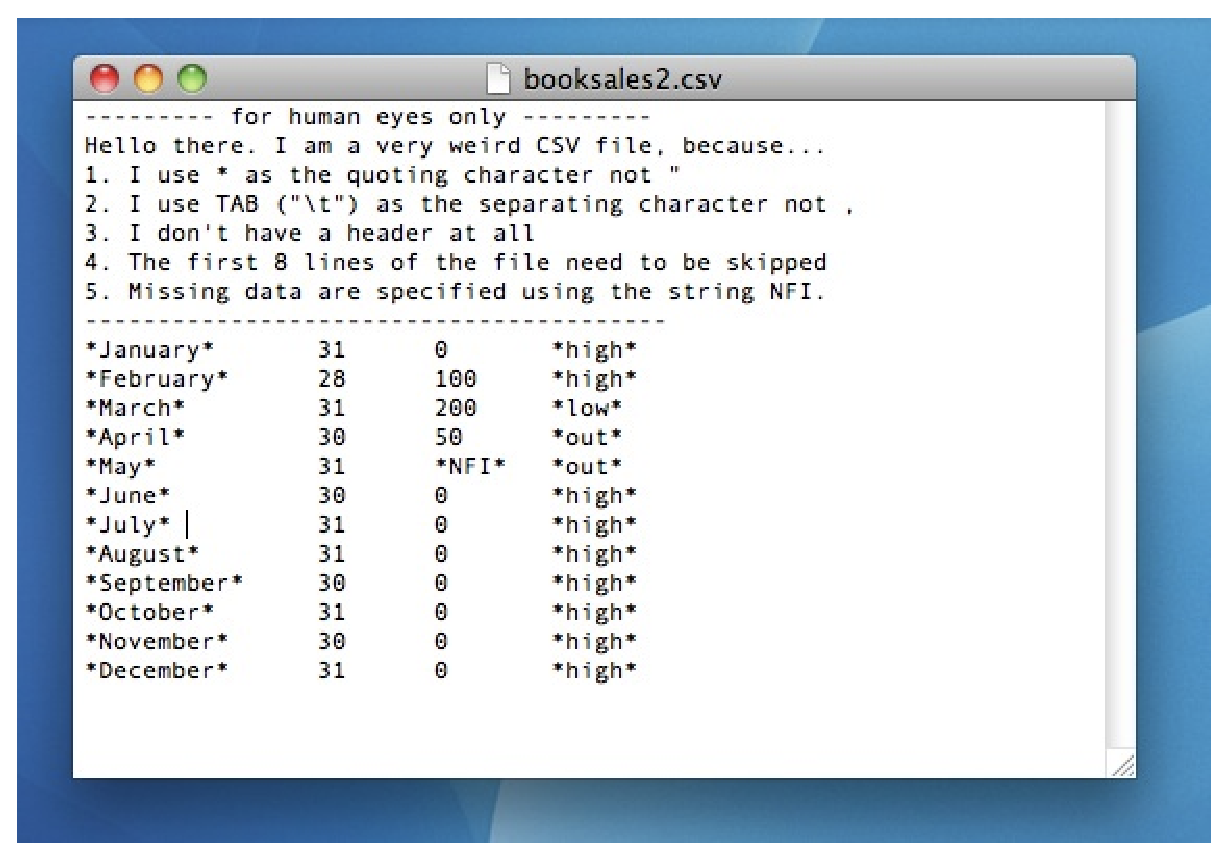
\epsfig{file = ../img/datahandling/booksales2csv.eps, clip=true,width = 14cm}
\caption{The \filename{booksales2.csv} data file. It contains more or less the same data as the original \filename{booksales.csv} data file, but has a lot of very quirky features.}
{#fig:booksales2csv}
\HR
\end{center}
\end{figure} 

In real life you'll rarely see data this stupidly formatted.^[If you're lucky.] 

### Loading data from SPSS (and other statistics packages)

The commands listed above are the main ones we'll need for data files in this book. But in real life we have many more possibilities. For example, you might want to read data files in from other statistics programs. Since SPSS is probably the most widely used statistics package in psychology, it's worth briefly showing how to open SPSS data files (file extension \filename{.sav}). It's surprisingly easy. The extract below should illustrate how to do so:
```
> library( foreign )                 # load the package
> X <- read.spss( "datafile.sav" )   # create a list containing the data
> X <- as.data.frame( X )            # convert to data frame
```
If you wanted to import from an SPSS file to a data frame directly, instead of importing a list and then converting the list to a data frame, you can do that too:
```
> X <- read.spss( file = "datafile.sav", to.data.frame = TRUE )
```
And that's pretty much it, at least as far as SPSS goes.  As far as other statistical software goes, the `foreign` package provides a wealth of possibilities. To open SAS files, check out the `read.ssd()`and `read.xport()` functions. To open data from Minitab, the `read.mtp()` function is what you're looking for. For Stata, the `read.dta()` function is what you want. For Systat, the `read.systat()` function is what you're after. 

### Loading Excel files 

A different problem is posed by Excel files. Despite years of yelling at people for sending data to me encoded in a proprietary data format, I get sent a lot of Excel files. In general R does a pretty good job of opening them, but it's bit finicky because Microsoft don't seem to be terribly fond of people using non-Microsoft products, and go to some lengths to make it tricky. If you get an Excel file, my suggestion would be to open it up in Excel (or better yet, OpenOffice, since that's free software) and then save the spreadsheet as a CSV file. Once you've got the data in that format, you can open it using `read.csv()`. However, if for some reason you're desperate to open the \filename{.xls} or \filename{.xlsx} file directly, then you can use the `read.xls()` function in the `gdata` package:
```
> library( gdata )                   # load the package
> X <- read.xls( "datafile.xlsx" )   # create a data frame
``` 
This usually works. And if it doesn't, you're probably justified in "suggesting" to the person that sent you the file that they should send you a nice clean CSV file instead.

### Loading Matlab (\& Octave) files 

A lot of scientific labs use Matlab as their default platform for scientific computing; or Octave as a free alternative. Opening Matlab data files (file extension \filename{.mat}) slightly more complicated, and if it wasn't for the fact that Matlab is so very widespread and is an extremely good platform, I wouldn't mention it. However, since Matlab is so widely used, I think it's worth discussing briefly how to get Matlab and R to play nicely together. The way to do this is to install the `R.matlab` package (don't forget to install the dependencies too). Once you've installed and loaded the package, you have access to the `readMat()` function. As any Matlab user will know, the \filename{.mat} files that Matlab produces are workspace files, very much like the \filename{.Rdata} files that R produces. So you can't import a \filename{.mat} file as a data frame. However, you can import it as a list. So, when we do this:
```
> library( R.matlab )                   # load the package
> data <- readMat( "matlabfile.mat" )   # read the data file to a list
```
The `data` object that gets created will be a list, containing one variable for every variable stored in the Matlab file. It's fairly straightforward, though there are some subtleties that I'm ignoring. In particular, note that if you don't have the `Rcompression` package, you can't open Matlab files above the version 6 format. So, if like me you've got a recent version of Matlab, and don't have the `Rcompression` package, you'll need to save your files using the \verb#-v6# flag otherwise R can't open them.


Oh, and Octave users? The `foreign` package contains a `read.octave()` command. Just this once, the world makes life easier for you folks than it does for all those cashed-up swanky Matlab bastards. 


### Saving other kinds of data

Given that I talked extensively about how to load data from non-R files, it might be worth briefly mentioning that R is also pretty good at writing data into other file formats besides it's own native ones. I won't discuss them in this book, but the `write.csv()` function can write CSV files, and the `write.foreign()` function (in the `foreign` package) can write SPSS, Stata and SAS files. There are also a lot of low level commands that you can use to write very specific information to a file, so if you really, really needed to you could create your own `write.obscurefiletype()` function, but that's also a long way beyond the scope of this book. For now, all that I want you to recognise is that this capability is there if you need it. 



### Are we done yet?

Of course not. If I've learned nothing else about R it's that you're *never bloody done*. This listing doesn't even come close to exhausting the possibilities. Databases are supported by the `RODBC`, `DBI`, and `RMySQL` packages among others. You can open webpages using the `RCurl` package. Reading and writing JSON objects is supported through the `rjson` package. And so on. In a sense, the right question is not so much "can R do this?" so much as "whereabouts in the wilds of CRAN *is* the damn package that does it?"









\section{Coercing data from one class to another{#coercion}}

Sometimes you want to change the variable class. This can happen for all sorts of reasons. Sometimes when you import data from files, it can come to you in the wrong format: numbers sometimes get imported as text, dates usually get imported as text, and many other possibilities besides. Regardless of how you've ended up in this situation, there's a very good chance that sometimes you'll want to convert a variable from one class into another one. Or, to use the correct term, you want to **_coerce_** the variable from one class into another. Coercion is a little tricky, and so I'll only discuss the very basics here, using a few simple examples. 

Firstly, let's suppose we have a variable `x` that is *supposed* to be representing a number, but the data file that you've been given has encoded it as text. Let's imagine that the variable is something like this:
```
> x <- "100"  # the variable 
> class(x)    # what class is it?
[1] "character"
```
Obviously, if I want to do calculations using `x` in its current state, R is going to get very annoyed at me. It thinks that `x` is text, so it's not going to allow me to try to do mathematics using it! Obviously, we need to coerce `x` from character to numeric. We can do that in a straightforward way by using the `as.numeric()` function: 
```
> x <- as.numeric(x)  # coerce the variable
> class(x)            # what class is it?
[1] "numeric"
> x + 1               # hey, addition works!
[1] 101
```
Not surprisingly, we can also convert it back again if we need to. The function that we use to do this is the `as.character()` function:
```
> x <- as.character(x)   # coerce back to text
> class(x)               # check the class:
[1] "character"
```
However, there's some fairly obvious limitations: you can't coerce the string `"hello world"` into a number because, well, there's isn't a number that corresponds to it. Or, at least, you can't do anything useful:
```
> as.numeric( "hello world" )  # this isn't going to work.
[1] NA
Warning message:
NAs introduced by coercion
```
In this case R doesn't give you an error message; it just gives you a warning, and then says that the data is missing (see Section@refsec:specials for the interpretation of `NA`). 

That gives you a feel for how to change between numeric and character data. What about logical data? To cover this briefly, coercing text to logical data is pretty intuitive: you use the `as.logical()` function, and the character strings `"T"`, `"TRUE"`, `"True"` and `"true"` all convert to the logical value of `TRUE`. Similarly `"F"`, `"FALSE"`, `"False"`, and `"false"` all become `FALSE`. All other strings convert to `NA`. When you go back the other way using `as.character()`, `TRUE` converts to `"TRUE"` and `FALSE` converts to `"FALSE"`. Converting numbers to logicals -- again using `as.logical()` -- is straightforward. Following the convention in the study of logic, the number `0` converts to `FALSE`. Everything else is `TRUE`. Going back using `as.numeric()`, `FALSE` converts to `0` and `TRUE` converts to `1`.


\section{Other useful data structures {#datastructures}}

Up to this point we have encountered several different kinds of variables. At the simplest level, we've seen numeric data, logical data and character data. However, we've also encountered some more complicated kinds of variables, namely factors, formulas, data frames and lists. We'll see a few more specialised data structures later on in this book, but there's a few more generic ones that I want to talk about in passing. None of them are central to the rest of the book (and in fact, the only one we'll even see anywhere else is the matrix), but they do crop up a fair bit in real life. 



### Matrices {#matrix (and arrays)}

In various different places in this chapter I've made reference to an R data structure called a **_matrix_**, and mentioned that I'd talk a bit more about matrices later on. That time has come. Much like a data frame, a matrix is basically a big rectangular table of data, and in fact there are quite a few similarities between the two. However, there are also some key differences, so it's important to talk about matrices in a little detail. Let's start by using `rbind()` to create a small matrix:^[You can also use the `matrix()` command itself, but I think the "binding" approach is a little more intuitive.]
```
> row.1 <- c( 2,3,1 )         # create data for row 1
> row.2 <- c( 5,6,7 )         # create data for row 2
> M <- rbind( row.1, row.2 )  # row bind them into a matrix
> print( M )                  # and print it out...
      [,1] [,2] [,3]
row.1    2    3    1
row.2    5    6    7
```
The variable `M` is a matrix, which we can confirm by using the `class()` function. Notice that, when we bound the two vectors together, R retained the names of the original variables as row names. We could delete these if we wanted by typing `rownames(M)<-NULL`, but I generally prefer having meaningful names attached to my variables, so I'll keep them. In fact, let's also add some highly unimaginative column names as well:
```
> colnames(M) <- c( "col.1", "col.2", "col.3" )
> print(M)
      col.1 col.2 col.3
row.1     2     3     1
row.2     5     6     7
```
You can use square brackets to subset a matrix in much the same way that you can for data frames, again specifying a row index and then a column index. For instance, `M[2,3]` pulls out the entry in the 2nd row and 3rd column of the matrix (i.e., `7`), whereas `M[2,]` pulls out the entire 2nd row, and `M[,3]` pulls out the entire 3rd column. However, it's worth noting that when you pull out a column, R will print the results horizontally, not vertically. The reason for this relates to how matrices (and arrays generally) are implemented. The original matrix `M` is treated as a two-dimensional objects, containing 2 rows and 3 columns. However, whenever you pull out a single row or a single column, the result is considered to be one-dimensional. As far as R is concerned there's no real reason to distinguish between a one-dimensional object printed vertically (a column) and a one-dimensional object printed horizontally (a row), and it prints them all out horizontally.^[This has some interesting implications for how matrix algebra is implemented in R (which I'll admit I initially found odd), but that's a little beyond the scope of this book. However, since there will be a small proportion of readers that do care, I'll quickly outline the basic thing you need to get used to: when multiplying a matrix by a vector (or one-dimensional array) using the `\%*\%` operator R will attempt to interpret the vector (or 1D array) as either a row-vector or column-vector, depending on whichever one makes the multiplication work. That is, suppose $\mathbf{M]$ is the $2\times3$ matrix, and $\bm{v}$ is a $1 \times 3$ row vector. It is impossible to multiply $\mathbf{M} \bm{v}$, since the dimensions don't conform, but you *can* multiply by the corresponding column vector, $\mathbf{M} \bm{v}^\T$. So, if I set ` v <- M[2,]` and then try to calculate `M \%*\% v`, which you'd think would fail, it actually works because R treats the one dimensional array as if it were a column vector for the purposes of matrix multiplication. Note that if both objects are one dimensional arrays/vectors, this leads to ambiguity since $\bm{v}\bm{v}^\T$ (inner product) and $\bm{v}^\T\bm{v}$ (outer product) yield different answers. In this situation, the `\%*\%` operator returns the inner product not the outer product. To understand all the details, check out the help documentation.} There is also a way of using only a single index, but due to the internal structure to how R defines a matrix, it works very differently to what we saw previously with data frames. The single-index approach is illustrated in Table@reftab:matrixindex but I don't really want to focus on it since we'll never really need it for this book, and matrices don't play anywhere near as large a role in this book as data frames do.

\begin{table}[t]
\begin{center}
\caption{An illustration of two different ways of indexing a $2 \times 3$ matrix. On the left we see the row and column version, which is identical to the corresponding indexing scheme for a data frame of the same size. On the right we see the single-index version, which is quite different to what we would get with a data frame. The reason for this is that, for both data frames and matrices, the "row and column" version exists to allow the human user to interact with the object in the psychologically meaningful way: since both data frames and matrices are basically just tables of data, it's the same in each case. However, the single-index version is really a method for you to interact with the object in terms of its internal structure, and the internals for data frames and matrices are quite different.}\tabcapsep
{#tab:matrixindex}
\begin{tabular}{ccc}
\begin{tabular}{c|ccc}
& \multicolumn{3}{c}{column} \\
row & 1 & 2 & 3 \\ \hline
1 & `[1,1]` & `[1,2]` & `[1,3]` \\
2 & `[2,1]` & `[2,2]` & `[2,3]` \\
\end{tabular}
&
\hspace*{1cm}
&
\begin{tabular}{c|ccc}
& \multicolumn{3}{c}{column} \\
row & 1 & 2 & 3 \\ \hline
1 & `[1]` & `[3]` & `[5]` \\
2 & `[2]` & `[4]` & `[6]` \\
\end{tabular}
\end{tabular}
\tabcapsep \HR
\end{center}
\end{table}


The critical difference between a data frame and a matrix is that, in a data frame, we have this notion that each of the columns corresponds to a different variable: as a consequence, the columns in a data frame can be of different data types. The first column could be numeric, and the second column could contain character strings, and the third column could be logical data. In that sense, there is a fundamental asymmetry build into a data frame, because of the fact that columns represent variables (which can be qualitatively different to each other) and rows represent cases (which cannot). Matrices are intended to be thought of in a different way. At a fundamental level, a matrix really is just *one* variable: it just happens that this one variable is formatted into rows and columns. If you want a matrix of numeric data, every single element in the matrix *must* be a number. If you want a matrix of character strings, every single element in the matrix *must* be a character string. If you try to mix data of different types together, then R will either spit out an error, or quietly coerce the underlying data into a list. If you want to find out what class R secretly thinks the data within the matrix is, you need to do something like this: 
```
> class( M[1] )
[1] "numeric"
```
You can't type `class(M)`, because all that will happen is R will tell you that `M` is a matrix: we're not interested in the class of the matrix itself, we want to know what class the underlying data is assumed to be. Anyway, to give you a sense of how R enforces this, let's try to change one of the elements of our numeric matrix into a character string:
```
> M[1,2] <- "text"
> M
      col.1 col.2  col.3
row.1 "2"   "text" "1"  
row.2 "5"   "6"    "7" 
```
It looks as if R has coerced all of the data in our matrix into character strings. And in fact, if we now typed in `class(M[1])` we'd see that this is exactly what has happened. If you alter the contents of one element in a matrix, R will change the underlying data type as necessary. 

There's only one more thing I want to talk about regarding matrices. The concept behind a matrix is very much a mathematical one, and in mathematics a matrix is a most definitely a two-dimensional object. However, when doing data analysis, we often have reasons to want to use higher dimensional tables (e.g., sometimes you need to cross-tabulate three variables against each other). You can't do this with matrices, but you can do it with **_arrays_**. An array is just like a matrix, except it can have more than two dimensions if you need it to. In fact, as far as R is concerned a matrix is just a special kind of array, in much the same way that a data frame is a special kind of list. I don't want to talk about arrays too much, but I will very briefly show you an example of what a 3D array looks like. To that end, let's cross tabulate the `speaker` and `utterance` variables from the \filename{nightgarden.Rdata} data file, but we'll add a third variable to the cross-tabs this time, a logical variable which indicates whether or not I was still awake at this point in the show:
```
> dan.awake <- c( TRUE,TRUE,TRUE,TRUE,TRUE,FALSE,FALSE,FALSE,FALSE,FALSE )
```
Now that we've got all three variables in the workspace (assuming you loaded the \filename{nightgarden.Rdata} data earlier in the chapter) we can construct our three way cross-tabulation, using the `table()` function. 
```
> xtab.3d <- table( speaker, utterance, dan.awake )
> xtab.3d
, , dan.awake = FALSE

             utterance
speaker       ee onk oo pip
  makka-pakka  0   2  0   2
  tombliboo    0   0  1   0
  upsy-daisy   0   0  0   0

, , dan.awake = TRUE

             utterance
speaker       ee onk oo pip
  makka-pakka  0   0  0   0
  tombliboo    1   0  0   0
  upsy-daisy   0   2  0   2
```
Hopefully this output is fairly straightforward: because R can't print out text in three dimensions, what it does is show a sequence of 2D slices through the 3D table. That is, the `, , dan.awake = FALSE` part indicates that the 2D table that follows below shows the 2D cross-tabulation of `speaker` against `utterance` only for the `dan.awake = FALSE` instances, and so on.^[I should note that if you type `class(xtab.3d)` you'll discover that this is a `"table"` object rather than an `"array"` object. However, this labelling is only skin deep. The underlying data structure here is actually an array. Advanced users may wish to check this using the command `class(unclass(xtab.3d))`, but it's not important for our purposes. All I really want to do in this section is show you what the output looks like when you encounter a 3D array.]


### Ordered factors {#orderedfactors}

One topic that I neglected to mention when discussing factors previously (Section@refsec:factors) is that there are actually two different types of factor in R, unordered factors and ordered factors. An unordered factor corresponds to a nominal scale variable, and all of the factors we've discussed so far in this book have been unordered (as will all the factors used anywhere else except in this section). However, it's often very useful to explicitly tell R that your variable is *ordinal scale*, and if so you need to declare it to be an **_ordered factor_**. For instance, earlier in this chapter we made use of a variable consisting of Likert scale data, which we represented as the `likert.raw` variable:
```
> likert.raw
 [1] 1 7 3 4 4 4 2 6 5 5
```
We can declare this to be an ordered factor in by using the `factor()` function, and setting `ordered = TRUE`. To illustrate how this works, let's create an ordered factor called `likert.ordinal` and have a look at it:
```
> likert.ordinal <- factor( x = likert.raw,        # the raw data 
+                           levels = seq(7,1,-1),  # strongest agreement is 1, weakest is 7
+                           ordered = TRUE )       # and it's ordered
> print( likert.ordinal )
 [1] 1 7 3 4 4 4 2 6 5 5
Levels: 7 < 6 < 5 < 4 < 3 < 2 < 1
```
Notice that when we print out the ordered factor, R explicitly tells us what order the levels come in. Because I wanted to order my levels in terms of *increasing* strength of agreement, and because a response of 1 corresponded to the strongest agreement and 7 to the strongest disagreement, it was important that I tell R to encode 7 as the lowest value and 1 as the largest. Always check this when creating an ordered factor: it's very easy to accidentally encode your data "upside down" if you're not paying attention. In any case, note that we can (and should) attach meaningful names to these factor levels by using the `levels()` function, like this:
```
> levels( likert.ordinal ) <- c( "strong.disagree", "disagree", "weak.disagree", 
+                                "neutral", "weak.agree", "agree", "strong.agree" )
> print( likert.ordinal )
 [1] strong.agree    strong.disagree weak.agree      neutral         neutral         neutral        
 [7] agree           disagree        weak.disagree   weak.disagree  
Levels: strong.disagree < disagree < weak.disagree < neutral < weak.agree < agree < strong.agree
```
One nice thing about using ordered factors is that there are a lot of analyses for which R automatically treats ordered factors differently from unordered factors, and generally in a way that is more appropriate for ordinal data. However, since I don't discuss that in this book, I won't go into details. Like so many things in this chapter, my main goal here is to make you aware that R has this capability built into it; so if you ever need to start thinking about ordinal scale variables in more detail, you have at least some idea where to start looking!




### Dates and times {#dates}

Times and dates are very annoying types of data. To a first approximation we can say that there are 365 days in a year, 24 hours in a day, 60 minutes in an hour and 60 seconds in a minute, but that's not quite correct. The length of the solar day is not exactly 24 hours, and the length of solar year is not exactly 365 days, so we have a complicated system of corrections that have to be made to keep the time and date system working. On top of that, the measurement of time is usually taken relative to a local time zone, and most (but not all) time zones have both a standard time and a daylight savings time, though the date at which the switch occurs is not at all standardised. So, as a form of data, times and dates *suck*. Unfortunately, they're also important. Sometimes it's possible to avoid having to use any complicated system for dealing with times and dates. Often you just want to know what year something happened in, so you can just use numeric data: in quite a lot of situations something as simple as `this.year <- 2011` works just fine. If you can get away with that for your application, this is probably the best thing to do. However, sometimes you really do need to know the actual date. Or, even worse, the actual time. In this section, I'll very briefly introduce you to the basics of how R deals with date and time data. As with a lot of things in this chapter, I won't go into details because I don't use this kind of data anywhere else in the book. The goal here is to show you the basics of what you need to do if you ever encounter this kind of data in real life. And then we'll all agree never to speak of it again.

To start with, let's talk about the date. As it happens, modern operating systems are very good at keeping track of the time and date, and can even handle all those annoying timezone issues and daylight savings pretty well. So R takes the quite sensible view that it can just ask the operating system what the date is. We can pull the date using the `Sys.Date()` function:
```
> today <- Sys.Date()  # ask the operating system for the date
> print(today)         # display the date
[1] "2011-08-24"
```
Okay, that seems straightforward. But, it does rather look like `today` is just a character string, doesn't it? That would be a problem, because dates really do have a numeric character to them, and it would be nice to be able to do basic addition and subtraction to them. Well, fear not. If you type in `class(today)`, R will tell you that the class of the `today` variable is `"Date"`. What this means is that, hidden underneath this text string that prints out an actual date, R actually has a numeric representation.^[Date objects are coded as the number of days that have passed since January 1, 1970.] What that means is that you actually can add and subtract days. For instance, if we add 1 to `today`, R will print out the date for tomorrow:
```
> today + 1
[1] "2011-08-25"
```
Let's see what happens when we add 365 days:
```
> today + 365
[1] "2012-08-23"
```
It turns out that R handles this better than I would have, since I'd forgotten that 2012 is a leap year and so I would have gotten the wrong answer had I done it myself. R provides a number of functions for working with dates, but I don't want to talk about them in any detail. I will, however, make passing mention of the `weekdays()` function which will tell you what day of the week a particular date corresponded to, which is extremely convenient in some situations:
``` 
> weekdays( today )
[1] "Wednesday"
```
I'll also point out that you can use the `as.Date()` to convert various different kinds of data into dates. If the data happen to be strings formatted exactly according to the international standard notation (i.e., \textsc{yyyy-mm-dd}) then the conversion is straightforward, because that's the format that R expects to see by default. You can convert dates from other formats too, but it's slightly trickier, and beyond the scope of this book.

What about times? Well, times are even more annoying, so much so that I don't intend to talk about them at all in this book, other than to point you in the direction of some vaguely useful things. R itself does provide you with some tools for handling time data, and in fact there are two separate classes of data that are used to represent times, known by the odd names `POSIXct` and `POSIXlt`. You can use these to work with times if you want to, but for most applications you would probably be better off downloading the `chron` package, which provides some much more user friendly tools for working with times and dates. 





\section{Miscellaneous topics {#miscdatahandling}}

To finish this chapter, I have a few topics to discuss that don't really fit in with any of the other things in this chapter. They're all kind of useful things to know about, but they are really just "odd topics" that don't fit with the other examples. Here goes:

### The problems with floating point arithmetic

If I've learned nothing else about transfinite arithmetic (and I haven't) it's that infinity is a tedious and inconvenient concept. Not only is it annoying and counterintuitive at times, but it has nasty practical consequences. As we were all taught in high school, there are some numbers that *cannot* be represented as a decimal number of finite length, nor can they be represented as any kind of fraction between two whole numbers; $\sqrt{2}$, $\pi$ and $e$, for instance. In everyday life we mostly don't care about this. I'm perfectly happy to approximate $\pi$ as 3.14, quite frankly. Sure, this does produce some rounding errors from time to time, and if I'd used a more detailed approximation like 3.1415926535 I'd be less likely to run into those issues, but in all honesty I've never needed my calculations to be *that* precise. In other words, although our pencil and paper calculations cannot represent the number $\pi$ exactly as a decimal number, we humans are smart enough to realise that we don't care. Computers, unfortunately, are dumb ... and you don't have to dig too deep in order to run into some very weird issues that arise because they can't represent numbers perfectly. Here is my favourite example: 
```
> 0.1 + 0.2 == 0.3
[1] FALSE
```
Obviously, R has made a mistake here, because this is definitely the wrong answer. Your first thought might be that R is broken, and you might be considering switching to some other language. But you can reproduce the same error in dozens of different programming languages, so the issue isn't specific to R. Your next thought might be that it's something in the hardware, but you can get the same mistake on any machine. It's something deeper than that. 

The fundamental issue at hand is **_floating point arithmetic_**, which is a fancy way of saying that computers will *always* round a number to fixed number of significant digits. The exact number of significant digits that the computer stores isn't important to us:^[For advanced users: type `?double` for more information.] what matters is that whenever the number that the computer is trying to store is very long, you get rounding errors. That's actually what's happening with our example above. There are teeny tiny rounding errors that have appeared in the computer's storage of the numbers, and these rounding errors have in turn caused the internal storage of `0.1 + 0.2` to be a tiny bit different from the internal storage of `0.3`. How big are these differences? Let's ask R:
```
> 0.1 + 0.2 - 0.3
[1] 5.551115e-17
```
Very tiny indeed. No sane person would care about differences that small. But R is not a sane person, and the equality operator `==` is very literal minded. It returns a value of `TRUE` only when the two values that it is given are absolutely identical to each other. And in this case they are not. However, this only answers half of the question. The other half of the question is, why are we getting these rounding errors when we're only using nice simple numbers like 0.1, 0.2 and 0.3? This seems a little counterintuitive. The answer is that, like most programming languages, R doesn't store numbers using their *decimal* expansion (i.e., base 10: using digits 0, 1, 2 ..., 9). We humans like to write our numbers in base 10 because we have 10 fingers. But computers don't have fingers, they have transistors; and transistors are built to store 2 numbers not 10. So you can see where this is going: the internal storage of a number in R is based on its *binary* expansion (i.e., base 2: using digits 0 and 1). And unfortunately, here's what the binary expansion of 0.1 looks like:
$$
.1 \mbox{(decimal)} = .00011001100110011... \mbox{(binary)} 
$$ 
and the pattern continues forever. In other words, from the perspective of your computer, which likes to encode numbers in binary,^[Or at least, that's the default. If all your numbers are integers (whole numbers), then you can explicitly tell R to store them as integers by adding an `L` suffix at the end of the number. That is, an assignment like `x <- 2L` tells R to assign `x` a value of 2, and to store it as an integer rather than as a binary expansion. Type `?integer` for more details.] 0.1 is not a simple number at all. To a computer, 0.1 is actually an infinitely long binary number! As a consequence, the computer can make minor errors when doing calculations here. 

With any luck you now understand the problem, which ultimately comes down to the twin fact that (1) we usually think in decimal numbers and computers usually compute with binary numbers, and (2) computers are finite machines and can't store infinitely long numbers. The only questions that remain are when you should care and what you should do about it. Thankfully, you don't have to care very often: because the rounding errors are small, the only practical situation that I've seen this issue arise for is when you want to test whether an arithmetic fact holds exactly numbers are identical (e.g., is someone's response time equal to *exactly* $2 \times 0.33$ seconds?) This is pretty rare in real world data analysis, but just in case it does occur, it's better to use a test that allows for a small *tolerance*. That is, if the difference between the two numbers is below a certain threshold value, we deem them to be equal for all practical purposes. For instance, you could do something like this, which asks whether the difference between the two numbers is less than a tolerance of $10^{-10}$
```
> abs( 0.1 + 0.2 - 0.3 ) < 10^-10
[1] TRUE
```
To deal with this problem, there is a function called `all.equal()` that lets you test for equality but allows a small tolerance for rounding errors:
```
> all.equal( 0.1 + 0.2, 0.3 )
[1] TRUE
```




### The recycling rule {#recycling}

There's one thing that I haven't mentioned about how vector arithmetic works in R, and that's the **_recycling rule_**. The easiest way to explain it is to give a simple example. Suppose I have two vectors of different length, `x` and `y`, and I want to add them together. It's not obvious what that actually means, so let's have a look at what R does:
```
> x <- c( 1,1,1,1,1,1 )  # x is length 6
> y <- c( 0,1 )          # y is length 2
> x + y                  # now add them:
[1] 1 2 1 2 1 2
```
As you can see from looking at this output, what R has done is "recycle" the value of the shorter vector (in this case `y`) several times. That is, the first element of `x` is added to the first element of `y`, and the second element of `x` is added to the second element of `y`. However, when R reaches the third element of `x` there isn't any corresponding element in `y`, so it returns to the beginning: thus, the third element of `x` is added to the *first* element of `y`. This process continues until R reaches the last element of `x`. And that's all there is to it really. The same recycling rule also applies for subtraction, multiplication and division. The only other thing I should note is that, if the length of the longer vector isn't an exact multiple of the length of the shorter one, R still does it, but also gives you a warning message:
```
> x <- c( 1,1,1,1,1 )    # x is length 5
> y <- c( 0,1 )          # y is length 2
> x + y                  # now add them:
[1] 1 2 1 2 1
Warning message:
In x + y : longer object length is not a multiple of shorter object length
```


### An introduction to environments {#environments}


\begin{figure}[t]
\begin{center}
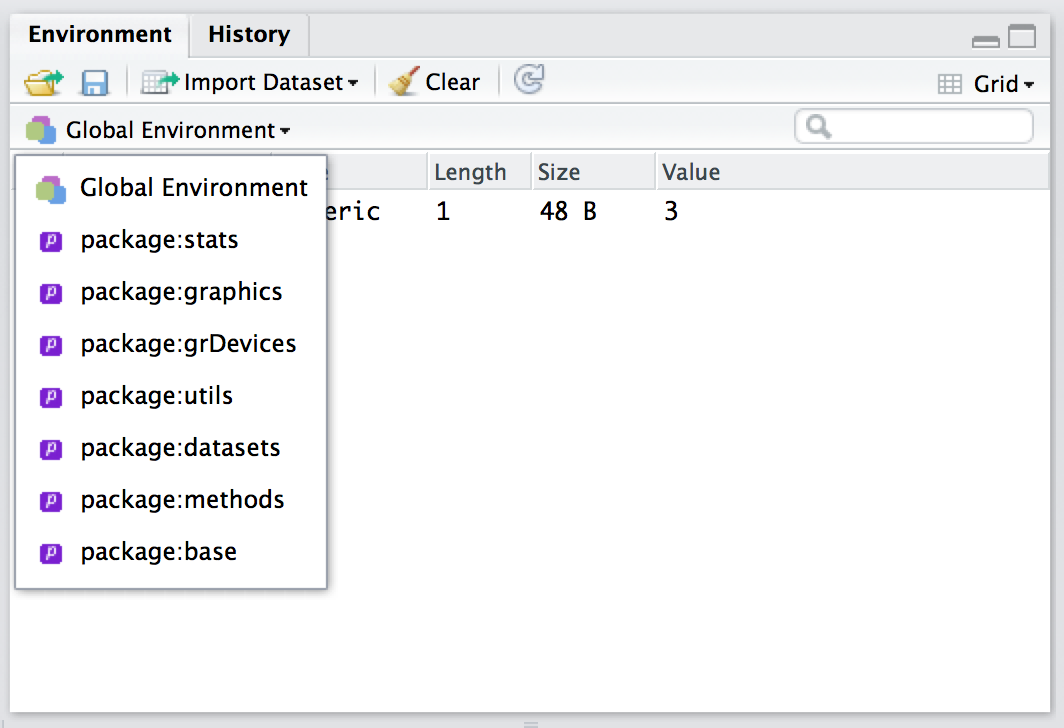
\epsfig{file = ../img/datahandling/environments.eps, clip=true,width = 10cm}
\caption{The environment panel in Rstudio can actually show you the contents of any loaded package: each package defines a separate environment, so you can select the one you want to look at in this panel.}
{#fig:envs}
\HR
\end{center}
\end{figure} 


In this section I want to ask a slightly different question: what *is* the workspace exactly? This question seems simple, but there's a fair bit to it. This section can be skipped if you're not really interested in the technical details. In the description I gave earlier, I talked about the workspace as an abstract location in which R variables are stored. That's basically true, but it hides a couple of key details. For example, any time you have R open, it has to store *lots* of things in the computer's memory, not just your variables. For example, the `who()` function that I wrote has to be stored in memory somewhere, right? If it weren't I wouldn't be able to use it. That's pretty obvious. But equally obviously it's not in the workspace either, otherwise you should have seen it! Here's what's happening. R needs to keep track of a lot of different things, so what it does is organise them into **_environments_**, each of which can contain lots of different variables and functions. Your workspace is one such environment. Every package that you have loaded is another environment. And every time you call a function, R briefly creates a temporary environment in which the function itself can work, which is then deleted after the calculations are complete. So, when I type in `search()` at the command line
```
> search()
 [1] ".GlobalEnv"        "package:lsr"       "tools:rstudio"    
 [4] "package:stats"     "package:graphics"  "package:grDevices"
 [7] "package:utils"     "package:datasets"  "package:methods"  
[10] "Autoloads"         "package:base"    
```
what I'm actually looking at is a *sequence of environments*. The first one, `".GlobalEnv"` is the technically-correct name for your workspace. No-one really calls it that: it's either called the workspace or the global environment. And so when you type in `objects()` or `who()` what you're really doing is listing the contents of `".GlobalEnv"`. But there's no reason why we can't look up the contents of these other environments using the `objects()` function (currently `who()` doesn't support this). You just have to be a bit more explicit in your command. If I wanted to find out what is in the `package:stats` environment (i.e., the environment into which the contents of the `stats` package have been loaded), here's what I'd get
```
> objects("package:stats")
  [1] "acf"                  "acf2AR"               "add.scope"           
  [4] "add1"                 "addmargins"           "aggregate"           
  [7] "aggregate.data.frame" "aggregate.default"    "aggregate.ts"        
 [10] "AIC"                  "alias"                "anova"               
 [13] "anova.glm"            "anova.glmlist"        "anova.lm"         
BLAH BLAH BLAH
```
where this time I've hidden a lot of output in the `BLAH BLAH BLAH` because the stats package contains about 500 functions. In fact, you can actually use the environment panel in Rstudio to browse any of your loaded packages (just click on the text that says "Global Environment" and you'll see a dropdown menu like the one shown in Figure@reffig:envs). The key thing to understand then, is that you can access any of the R variables and functions that are stored in one of these environments, precisely because those are the environments that you have loaded!^[For advanced users: that's a little over simplistic in two respects. First, it's a terribly imprecise way of talking about scoping. Second, it might give you the impression that all the variables in question are actually loaded into memory. That's not quite true, since that would be very wasteful of memory. Instead R has a "lazy loading" mechanism, in which what R actually does is create a "promise" to load those objects if they're actually needed. For details, check out the `delayedAssign()` function.] 


### Attaching a data frame

The last thing I want to mention in this section is the `attach()` function, which you often see referred to in introductory R books. Whenever it is introduced, the author of the book usually mentions that the `attach()` function can be used to "attach" the data frame to the search path, so you don't have to use the \rtextverb#$# operator. That is, if I use the command `attach(df)` to attach my data frame, I no longer need to type \rtextverb#df$variable#, and instead I can just type `variable`. This is true as far as it goes, but it's very misleading and novice users often get led astray by this description, because it hides a lot of critical details. 

Here is the very abridged description: when you use the `attach()` function, what R does is create an entirely new *environment* in the search path, just like when you load a package. Then, what it does is *copy* all of the variables in your data frame into this new environment. When you do this, however, you end up with two completely different versions of all your variables: one in the original data frame, and one in the new environment. Whenever you make a statement like \rtextverb#df$variable# you're working with the variable inside the data frame; but when you just type `variable` you're working with the copy in the new environment. And here's the part that really upsets new users: *changes to one version are not reflected in the other version*. As a consequence, it's really easy for R to end up with different value stored in the two different locations, and you end up really confused as a result. 

To be fair to the writers of the `attach()` function, the help documentation does actually state all this quite explicitly, and they even give some examples of how this can cause confusion at the bottom of the help page. And I can actually see how it can be very useful to create copies of your data in a separate location (e.g., it lets you make all kinds of modifications and deletions to the data without having to touch the original data frame). However, I don't think it's helpful for new users, since it means you have to be very careful to keep track of which copy you're talking about. As a consequence of all this, for the purpose of this book I've decided not to use the `attach()` function. It's something that you can investigate yourself once you're feeling a little more confident with R, but I won't do it here. 




\section{Summary}

Obviously, there's no real coherence to this chapter. It's just a grab bag of topics and tricks that can be handy to know about, so the best wrap up I can give here is just to repeat this list:

 \itemsep 0pt
\item Section@refsec:freqtables. Tabulating data.
\item Section@refsec:transform. Transforming or recoding a variable.
\item Section@refsec:mathfunc. Some useful mathematical functions.
\item Section@refsec:subset. Extracting a subset of a vector.
\item Section@refsec:subsetdataframe. Extracting a subset of a data frame.
\item Section@refsec:sort. Sorting, flipping or merging data sets.
\item Section@refsec:reshape. Reshaping a data frame.
\item Section@refsec:textprocessing. Manipulating text.
\item Section@refsec:importing. Opening data from different file types.
\item Section@refsec:coercion. Coercing data from one type to another.
\item Section@refsec:datastructures. Other important data types.
\item Section@refsec:miscdatahandling. Miscellaneous topics.


There are a number of books out there that extend this discussion. A couple of my favourites are \citeA{Spector2008} "Data Manipulation with R" and \citeA{Teetor2011} "R Cookbook". 







